\motto{In den Dreißiger Jahren besuchte ich regelmäßig die Schweiz, teils um mich auch auf den Viertausendern zu tummeln, zum großen Teil aber auch, um Emigrantenblätter zu lesen und mich mit Kollegen über Naziverbrechen zu unterhalten. Aber auch die Schweizer schauten sich, wenn sie offen reden wollten, ebenso ängstlich um wie das bei uns üblich war.\footnote{The \href{https://www.universityworldnews.com/post.php?story=20241107142108558}{recent policy of ETH} against Chinese students makes me feel that nothing has changed in Switzerland after the collapsing of Nazi for almost 80 years.}

--- Oskar Perron\footnote{Oskar Perron (1880--1975), after earning an \emph{Eisernes Kreuz} during WWI, obtained a position in München in 1922, initiating the glorious period there. Among his colleagues were Carathéodory, Tietze and Sommerfield.}}
\chapter{Geodesic rays in the space of potentials}
\label{chap:rays}

When $\omega$ is a K\"ahler form, the space of smooth strictly $\omega$-plurisubharmonic potentials carries the Mabuchi $L^2$-metric. Its geodesic equation is the homogeneous complex Monge--Amp\`ere equation on $X\times\{0<\Real z<1\}$. Subsolutions of this equation are subgeodesics, and the geodesic between two boundary potentials is obtained as a Perron envelope. This construction continues to make sense for singular potentials, even when no smooth geodesic exists.

The goal of this chapter is to further develop the corresponding theory for $\theta$-plurisubharmonic potentials, where $\theta$ is a smooth closed real $(1,1)$-form representing a big class. We define subgeodesics by requiring the complexification $\Phi(x,z)=\varphi_{\Real z}(x)$ to be plurisubharmonic. Geodesics are then defined as Perron envelopes of subgeodesics with prescribed boundary values. This point of view is flexible enough to handle unbounded potentials and singularity constraints.

The first section sets up the basic properties of subgeodesics. We then construct geodesics with prescribed singular endpoints and study geodesic rays. The results are formulated relative to a model potential $\phi$, so that the endpoints and rays live in a fixed relative singularity class.

The final part of the chapter studies the finite-energy space $\mathcal E^1(X,\theta;\phi)$ and the Darvas $d_1$-metric. We prove the basic metric properties needed later, including completeness and monotone convergence criteria. The radial version of the metric on geodesic rays will be used in the study of test curves and singularity types.

This chapter provides the analytic bridge between envelopes and the later non-Archimedean theory. The space $\mathcal E^1(X,\theta;\phi)$ and the $d_1$-geometry developed here feed into the pseudometric $d_S$ of \cref{chap:comp}, while geodesic rays will later be related to test curves and non-Archimedean potentials.


\section{Subgeodesics}\label{sec:subgeo}
Let $X$ be a connected compact Kähler manifold of dimension $n$ and $\theta$ be a smooth closed real $(1,1)$-form on $X$ representing a big cohomology class.

\begin{definition}\label{def:subgeod}
    Let us fix $\varphi_0,\varphi_1\in \PSH(X,\theta)$. A \emph{subgeodesic}\index{subgeodesic} from $\varphi_0$ to $\varphi_1$ is a family $(\varphi_t)_{t\in (0,1)}$ in $\PSH(X,\theta)$ such that
    \begin{enumerate}
        \item\label{itm:def:subgeod:1} if we define
            \[
                \Phi\colon X\times \Bigl\{z\in \mathbb{C}:\Real z\in (0,1) \Bigr\}\rightarrow [-\infty,\infty),\quad (x,z)\mapsto \varphi_{\Real z}(x),
            \]
            then $\Phi$ is $p_1^*\theta$-psh, where $p_1\colon X\times \{z\in \mathbb{C}:\Real z\in (0,1)\}\rightarrow X$ is the natural projection;
        \item\label{itm:def:subgeod:2} when $t\to 0+$ (resp. $t\to 1-$), $\varphi_t$ converges to $\varphi_0$ (resp. $\varphi_1$) with respect to the $L^1$-topology.
    \end{enumerate}
    We also say $(\varphi_t)_{t\in [0,1]}$ is a subgeodesic.

    We call $\Phi$ the \emph{complexification}\index{complexification} of the subgeodesic $(\varphi_t)_t$.
\end{definition}
When we do not want to specify $\varphi_0$ and $\varphi_1$, we shall say $(\varphi_t)_{t\in (0,1)}$ is a subgeodesic\footnote{Note that it is implicit in the definition that $\varphi_t$ as $t\to 0+$ or $t\to 1-$ admits an $L^1$-limit.}.

More generally, a family $(\psi_t)_{t\in [a,b]}$ (resp. $(\psi_t)_{t\in (a,b)}$) in $\PSH(X,\theta)$ for some $a\leq b$ is called a \emph{subgeodesic}\index{subgeodesic} if $(\psi_{tb+(1-t)a})_{t\in [0,1]}$ (resp. $(\psi_{tb+(1-t)a})_{t\in (0,1)}$) is a subgeodesic.

\begin{remark}
    Note that given a subgeodesic $(\psi_t)_{t\in (a,b)}$, the endpoints $\psi_a$ and $\psi_b$ are uniquely determined, in view of \cref{prop:pshfuncdetdense}.
\end{remark}

\begin{remark}\label{rmk:complexify1}
In the literature, people sometimes regard $\Phi$ as a function defined on $X\times\{z\in \mathbb{C}: \mathrm{e}^{-1}<|z|<1\}$, with $\Phi(x,z)=\varphi_{-\log |z|}(x)$. We sometimes also use this convention; the ambient strip or annulus will make the convention clear.
\end{remark}



In general, there are no subgeodesics from $\varphi_0$ to $\varphi_1$. In fact, by \cref{prop:convexsubgeod} below, the existence of a subgeodesic from $\varphi_0$ to $\varphi_1$ forces $\varphi_0\land\varphi_1\not\equiv-\infty$, a condition that may fail (see \cref{ex:landminfty}).

We first note that the subgeodesics are well-behaved under the change of $\theta$:
\begin{proposition}\label{prop:subgeodindeptheta}
    Let $g$ be a smooth real function on $X$.
    Let $\theta'=\theta+\ddc g$. Suppose that $(\varphi_t)_{t\in [0,1]}$ is a subgeodesic in $\PSH(X,\theta)$. Then $(\varphi_t-g)_{t\in [0,1]}$ is a subgeodesic in $\PSH(X,\theta')$.
\end{proposition}
\begin{proof}
    This follows directly from the definition of the complexification.
\end{proof}

\begin{example}\label{ex:linearsubgeod}
    Let $\varphi_0\in \PSH(X,\theta)$, $C\in \mathbb{R}$. Let
    \[
    \varphi_t=\varphi_0+tC,\quad t\in [0,1].
    \]
    Then $(\varphi_t)_{t\in [0,1]}$ is a subgeodesic.
    Indeed, since $\Real z$ is harmonic in $z$, the complexification $\Phi(x,z)=\varphi_0(x)+C\,\Real z$ is $p_1^*\theta$-psh.

    As a consequence, the constant $(\varphi_0)_{t\in [0,1]}$ is a subgeodesic, called the \emph{constant subgeodesic}\index{subgeodesic!constant subgeodesic} at $\varphi_0$.

    A more general version is as follows: Suppose that $(\varphi_t)_{t\in [0,1]}$ is a subgeodesic in $\PSH(X,\theta)$, $C_1,C_2\in \mathbb{R}$. Then $(\varphi_t+C_1t+C_2)_{t\in [0,1]}$ is also a subgeodesic.
\end{example}


\begin{proposition}\label{prop:convexsubgeod}
    Let $\varphi_0,\varphi_1\in \PSH(X,\theta)$ and $(\varphi_t)_{t\in (0,1)}$ be a subgeodesic from $\varphi_0$ to $\varphi_1$. Then for each $x\in X$, $[0,1] \ni t\mapsto \varphi_t(x)$ is a convex function. Furthermore,
    \[
    \inf_{t\in (0,1)}\varphi_t\in \PSH(X,\theta),\quad \inf_{t\in (0,1)}\varphi_t\leq \varphi_0\land \varphi_1.
    \]
\end{proposition}


\begin{proof}
    Let $\Phi$ be the complexification of $(\varphi_t)_{t\in (0,1)}$.

    For each $x\in X$, the map
    \[
    \Bigl\{z\in \mathbb{C}: \Real z\in (0,1) \Bigr\}\rightarrow [-\infty,\infty),\quad z\mapsto \Phi(x,z)
    \]
    is either subharmonic or constantly $-\infty$, as follows from \itemref{itm:def:subgeod:1} and \cref{prop:pullbackpsh}.
    In the latter case, the convexity of $[0,1] \ni t\mapsto \varphi_t(x)$ is trivial. In the former case, the convexity on the interval $(0,1)$ follows from
    \cref{prop:subhimplyconv}.

    In order to verify the convexity at the boundary, let us fix $s\in (0,1)$. We need to show that
    \begin{equation}\label{eq:varphisconvextemp1}
    \varphi_s(x)\leq s\varphi_1(x)+(1-s)\varphi_0(x)
    \end{equation}
    for all $x\in X$. Thanks to \cref{prop:pshfuncdetdense}, it suffices to prove this for almost all $x$.

    Choose sequences $a_j\searrow0$ and $b_j\nearrow1$ such that $\varphi_{a_j}\to\varphi_0$ and $\varphi_{b_j}\to\varphi_1$ almost everywhere. Outside a set $Z\subseteq X$ of zero Lebesgue measure, all these convergences hold and all the values involved are finite. For $x\in X\setminus Z$ and $j$ large enough that $a_j<s<b_j$, the convexity on $(0,1)$ gives
    \[
    \varphi_s(x)\leq \frac{b_j-s}{b_j-a_j}\varphi_{a_j}(x)+\frac{s-a_j}{b_j-a_j}\varphi_{b_j}(x).
    \]
    Letting $j\to\infty$ gives \eqref{eq:varphisconvextemp1} almost everywhere.

    Let us prove the last assertion. Let
    \[
    \varphi\coloneqq \inf_{t\in (0,1)}\varphi_t.
    \]
    By Kiselman's principle \cref{prop:Kis}, we know that $\varphi\in \PSH(X,\theta)\cup \{-\infty\}$. Since the complexification $\Phi$ is not identically $-\infty$, Fubini's theorem shows that for almost every $x\in X$, the function $t\mapsto \varphi_t(x)$ is finite for almost every $t\in (0,1)$. For such an $x$, the convexity just proved implies that $t\mapsto \varphi_t(x)$ is a finite convex function on $(0,1)$, hence it is bounded from below on $(0,1)$. Thus $\varphi\not\equiv -\infty$, and so $\varphi\in \PSH(X,\theta)$.

    For any $t\in (0,1)$, using the convexity established above, we have
    \[
    \varphi\leq (1-t)\varphi_0+t\varphi_1.
    \]
    It follows that $\varphi\leq \varphi_0$ and $\varphi\leq \varphi_1$ almost everywhere and hence everywhere by \cref{prop:pshfuncdetdense}. Our assertion follows.
\end{proof}

\begin{corollary}\label{cor:subgeodboundary}
    Let $\varphi_0,\varphi_1\in \PSH(X,\theta)$ and $(\varphi_t)_{t\in (0,1)}$ be a subgeodesic from $\varphi_0$ to $\varphi_1$. Then
    \begin{equation}\label{eq:varphitconvexbdry}
    \lim_{t\to 0+}\varphi_t\leq \varphi_0,\quad   \lim_{t\to 1-}\varphi_t\leq \varphi_1.
    \end{equation}
    Moreover,
    \[
    \lim_{t\to 0+}\varphi_t=\varphi_0,\quad   \lim_{t\to 1-}\varphi_t=\varphi_1\quad \textup{quasi-everywhere}.
    \]
\end{corollary}
The inequalities in \eqref{eq:varphitconvexbdry} are not equalities everywhere in general. For example, consider an arbitrary subgeodesic from an unbounded $\varphi_0\in \mathcal{E}(X,\omega)$ to a bounded $\varphi_1\in \PSH(X,\omega)$ for some Kähler form $\omega$ on $X$.
\begin{proof}
    The inequalities in \eqref{eq:varphitconvexbdry} and the existence of the limits follow from the convexity in \cref{prop:convexsubgeod}. Let us prove the quasi-everywhere equality at $t=0$. Take a decreasing sequence $t_j\searrow 0$ with $t_j>0$. Then $\varphi_{t_j}\to \varphi_0$ in $L^1(X)$ as $j\to\infty$. So by \cref{cor:L1limipp}, we have
    \[
    \varlimsup_{j\to\infty}\varphi_{t_j}= \varphi_0\quad \textup{quasi-everywhere}.
    \]
    Therefore, we have
    \[
    \varphi_0=\varlimsup_{j\to\infty}\varphi_{t_j}=\lim_{t\to 0+}\varphi_t\leq \varphi_0\quad \textup{quasi-everywhere}.
    \]
    The assertion at $t=1$ is similar.
\end{proof}


\begin{corollary}\label{cor:convexsubgeod}
    Let $(\varphi_t)_{t\in [0,1]}$ be a subgeodesic in $\PSH(X,\theta)$. Then
    \begin{equation}\label{eq:supconvexsubgeod}
        \adjustlimits\sup_X \inf_{s\in (0,1)}\varphi_s \leq \sup_X \varphi_t\leq \sup_X \varphi_0\lor \sup_X \varphi_1
    \end{equation}
    for all $t\in (0,1)$.

    Furthermore, $[0,1] \ni t\mapsto \varphi_t$ is continuous with respect to the $L^1$-topology.
\end{corollary}
In particular, in view of \cref{prop:L1compa}, the family $\{\varphi_t\}_{t\in [0,1]}$ is relatively compact with respect to the $L^1$-topology on $\PSH(X,\theta)$.
\begin{proof}
    \eqref{eq:supconvexsubgeod} follows immediately from \cref{prop:convexsubgeod}.
    Let us verify the continuity of $t\mapsto \varphi_t$. The continuity at $t=0$ or $t=1$ follows from the definition of subgeodesic. While the continuity on $(0,1)$ follows from the convexity of $t\mapsto \varphi_t$, and the fact that $\varphi_t\in L^1(X)$ for each $t\in (0,1)$.
\end{proof}


\begin{proposition}\label{prop:maxsubgeod}
    Let $(\varphi^i_0)_{i\in I}$, $(\varphi^i_1)_{i\in I}$ be two non-empty uniformly bounded from above families in $\PSH(X,\theta)$. Let $(\varphi^i_t)_{t\in (0,1)}$ be subgeodesics from $\varphi_0^i$ to $\varphi_1^i$ for each $i\in I$. Then
    \[
    \left(\uscsup[i\in I]\varphi^i_t\right)_{t\in (0,1)}
    \]
    is a subgeodesic from $\uscsup[i] \varphi^i_0$ to $\uscsup[i] \varphi^i_1$.
\end{proposition}
\begin{proof}
    We may assume that $\varphi_0^i,\varphi_1^i\leq 0$ for all $i\in I$. Then it follows that $\varphi_t^i\leq 0$ for all $t\in (0,1)$ and all $i\in I$ by \cref{prop:convexsubgeod}.

    We define
    \[
    \varphi_t\coloneqq \uscsup[i\in I] \varphi^i_t\in \PSH(X,\theta)
    \]
    for all $t\in [0,1]$.
    Observe that $[0,1] \ni t\mapsto \varphi_t$ is convex by the same argument leading to \eqref{eq:varphisconvextemp1}.

    Let $(\psi_t)_{t\in (0,1)}$ be the subgeodesic whose complexification $\Phi_{\psi}$ corresponds to $\uscsup[i] \Phi_{\varphi^i}$, where $\Phi_{\varphi^i}$ is the complexification of $(\varphi^i_t)_{t\in (0,1)}$. Then clearly, $\varphi_t\leq \psi_t$ for each $t\in (0,1)$. On the other hand, by \cref{prop:supsupstardiff},
    \[
    \psi_t=\sup_{i\in I}\varphi^i_t=\varphi_t\quad \textup{almost everywhere}
    \]
    for almost all $t\in (0,1)$. Therefore, using \cref{prop:pshfuncdetdense}, we find $\psi_t=\varphi_t$ for almost all $t\in (0,1)$. Since both functions are convex in $t$, we conclude that $\psi_t=\varphi_t$ for all $t\in (0,1)$.

    It remains to argue that $\varphi_t\xrightarrow{L^1}\varphi_0$ as $t\to 0+$ and $\varphi_t\xrightarrow{L^1}\varphi_1$ as $t\to 1-$.
    By symmetry, it suffices to argue the former.

    By Choquet's lemma \cref{prop:Choquet}, applied to the uniformly bounded above family of complexifications $(\Phi_{\varphi^i})_{i\in I}$ on the strip, there is a countable subset $I'\subset I$ such that
    \[
    \uscsup[i\in I]\Phi_{\varphi^i}=\uscsup[i\in I']\Phi_{\varphi^i}.
    \]
    Applying Choquet's lemma \cref{prop:Choquet} once more to the endpoint families if necessary, and enlarging $I'$, we may also assume
    \[
    \uscsup[i\in I]\varphi_0^i=\uscsup[i\in I']\varphi_0^i,\quad \uscsup[i\in I]\varphi_1^i=\uscsup[i\in I']\varphi_1^i.
    \]
    Thus, after replacing $I$ by $I'$, we may assume that $I$ is countable.

    We know that for any $t\in (0,1)$ and any $j\in I$,
    \[
    \varphi^j_t\leq \varphi_t\leq t\varphi_1+(1-t)\varphi_0.
    \]
    Letting $t\to 0+$, we find that
    \[
    \varphi_0^j\leq \varlimsup_{t\to 0+}\varphi_t\leq \varphi_0
    \]
    almost everywhere. Since $I$ is countable, we conclude that
    \begin{equation}\label{eq:varphi0limsuptemp1}
    \varphi_0=\varlimsup_{t\to 0+}\varphi_t
    \end{equation}
    almost everywhere.

    Fix $i_0\in I$.
    Recall that by \cref{prop:convexsubgeod}, for each $t\in (0,1)$, we have
    \[
    \adjustlimits \inf_{t\in (0,1)}\sup_X \varphi_t\geq \adjustlimits\inf_{t\in (0,1)}\sup_X \varphi^{i_0}_t\geq \adjustlimits\sup_X \inf_{t\in (0,1)}\varphi^{i_0}_t>-\infty,
    \]
    so the set $\{\varphi_t\}_{t\in (0,1)}$ is relatively compact with respect to the $L^1$-topology by \cref{prop:L1compa}.
    Let $\psi$ be a cluster point as $t\to 0+$. It suffices to show that $\psi=\varphi_0$. By \cref{cor:L1limipp} and \eqref{eq:varphi0limsuptemp1}, this holds almost everywhere. Therefore, it holds everywhere by \cref{prop:pshfuncdetdense}.
\end{proof}

\begin{proposition}\label{prop:subgeodrestsubgeod}
    Let $(\varphi_t)_{t\in [0,1]}$ be a subgeodesic in $\PSH(X,\theta)$. Then for any $0\leq a\leq b\leq 1$, the segment $(\varphi_{t})_{t\in [a,b]}$ is a subgeodesic.
\end{proposition}



\begin{proof}
    It suffices to show that
    \[
    \varphi_{tb+(1-t)a}\xrightarrow{L^1}\varphi_a,\quad \varphi_{tb+(1-t)a}\xrightarrow{L^1}\varphi_b
    \]
    as $t\to 0+$ and $t\to 1-$ respectively. In other words, we need to show that for any $c\in (0,1)$, we have
    \[
    \varphi_t\xrightarrow{L^1}\varphi_c
    \]
    as $t\to c$. For this purpose, observe that by \cref{prop:convexsubgeod},
    \[
    \adjustlimits\sup_X \inf_{s\in (0,1)}\varphi_s\leq \sup_{X}\varphi_t\leq \left( \sup_X \varphi_0 \right) \lor \left( \sup_X\varphi_1 \right)
    \]
    for any $t\in (0,1)$. Therefore, $\{\varphi_t\}_{t\in (0,1)}$ is a relatively compact family with respect to the $L^1$-topology on $\PSH(X,\theta)$ by \cref{prop:L1compa}. It suffices to show that any cluster point $\psi$ of $\varphi_t$ as $t\to c$ is equal to $\varphi_c$.
    By \cref{cor:L1limipp} and the convexity \cref{prop:convexsubgeod}, we have $\varphi_c=\psi$ almost everywhere and hence everywhere by \cref{prop:pshfuncdetdense}.
\end{proof}

For the purpose of this chapter, it is useful to reformulate the gluing lemma \cref{cor:glbdry} in the following way, which allows us to glue subgeodesics directly:
\begin{lemma}\label{lma:subgeodgluing}
    Let $(\varphi_t)_{t\in [0,1]}$ be a subgeodesic in $\PSH(X,\theta)$. Let $0\leq a<b\leq 1$ and let $(\psi_t)_{t\in [a,b]}$ be a subgeodesic such that $\psi_a=\varphi_a$, $\psi_b=\varphi_b$, and
    \[
        \psi_t\geq \varphi_t,\quad t\in (a,b).
    \]
    Define
    \[
    \gamma_t=
    \begin{cases}
        \psi_t,&\textup{if }t\in (a,b),\\
        \varphi_t,&\textup{if }t\in [0,1]\setminus (a,b).
    \end{cases}
    \]
    Then $(\gamma_t)_{t\in [0,1]}$ is a subgeodesic.
\end{lemma}
\begin{proof}
    The $L^1$-convergence of $\gamma_t$ to $\varphi_0$ at $0$ and $\varphi_1$ at $1$ follows immediately from the corresponding property for $(\varphi_t)_t$ and $(\psi_t)_t$.
    It remains to prove that the complexification of $(\gamma_t)_t$ is $p_1^*\theta$-psh.

    Let
    \[
        S=\{z\in\mathbb{C}:0<\Real z<1\},\quad S'=\{z\in\mathbb{C}:a<\Real z<b\}.
    \]
    Let $\Phi$ and $\Psi$ be the complexifications of $(\varphi_t)_t$ and $(\psi_t)_t$ on the corresponding strips. Since $\Psi\geq \Phi$ on $X\times S'$, the complexification of $(\gamma_t)_t$ is equal to $\Phi\lor\Psi$ on $X\times S'$ and to $\Phi$ on $X\times (S\setminus S')$.
    By the gluing lemma \cref{cor:glbdry}, it is enough to verify that
    \[
        \varlimsup_{\substack{S'\ni z'\to z\\ x'\to x}}\Psi(x',z')\leq \Phi(x,z)
    \]
    at every point $(x,z)\in X\times S$ with $\Real z=a$ or $\Real z=b$.

    Suppose for instance that $a>0$, and let $(x_j,z_j)$ tend to $(x,z)$ with $\Real z=a$ and $a<\Real z_j<b$. Set $t_j=\Real z_j$. Since $(\psi_t)_t$ is a subgeodesic from $\varphi_a$ to $\varphi_b$, the sequence $\psi_{t_j}$ converges to $\varphi_a$ in $L^1$. Applying \cref{cor:L1limipp} to this sequence gives
    \[
        \varphi_a=\inf_{m>0}\left(\uscsup[j\geq m]\psi_{t_j}\right).
    \]
    For fixed $m$, the upper semicontinuity of $\uscsup[j\geq m]\psi_{t_j}$ gives
    \[
        \varlimsup_{j\to\infty}\psi_{t_j}(x_j)\leq \left(\uscsup[j\geq m]\psi_{t_j}\right)(x).
    \]
    Letting $m\to\infty$, we get
    \[
        \varlimsup_{j\to\infty}\psi_{t_j}(x_j)\leq \varphi_a(x).
    \]
    Since $\Phi(x,z)=\varphi_a(x)$ when $\Real z=a$, this is the desired boundary inequality along $\{\Real z=a\}$. The same argument applies along $\{\Real z=b\}$ when $b<1$. Hence \cref{cor:glbdry} shows that the pasted complexification is $p_1^*\theta$-psh.
\end{proof}

\begin{definition}\label{def:subgeoray}
    A ray $\ell=(\ell_t)_{t\geq 0}$ is a \emph{subgeodesic ray}\index{subgeodesic ray} in $\PSH(X,\theta)$ if for any $0\leq a\leq b$, the segment $(\ell_{t})_{t\in [a,b]}$ is a subgeodesic in $\PSH(X,\theta)$. We say $\ell$ \emph{emanates} from $\ell_0$.

    The \emph{complexification}\index{complexification} of a subgeodesic ray $\ell$ is defined as the potential
    \[
    \Phi\colon X\times \{z\in \mathbb{C}:\Real z>0\}\rightarrow [-\infty,\infty),\quad (x,z)\mapsto \ell_{\Real z}(x).
    \]
    Note that $\Phi$ is $p_1^*\theta$-psh, where $p_1\colon X\times \{z\in \mathbb{C}:\Real z>0\}\rightarrow X$ is the natural projection.
\end{definition}
\begin{remark}
    As in \cref{rmk:complexify1}, one may also define the complexification as a function $X\times \{z\in \mathbb{C}: 0<|z|<1\}\rightarrow [-\infty,\infty)$.
\end{remark}



\section{Geodesics in the space of potentials}\label{sec:relativeray}
Let $X$ be a connected compact Kähler manifold of dimension $n$ and $\theta$ be a smooth closed real $(1,1)$-form on $X$ representing a big cohomology class.
Fix a model potential $\phi\in \PSH(X,\theta)_{>0}$. See \cref{def:modelpot} for the definition.

\begin{definition}\label{def:geo}
    Let $\varphi_0, \varphi_1 \in \PSH(X,\theta)$. The \emph{geodesic}\index{geodesic} $(\varphi_t)_{t\in (0,1)}$ from $\varphi_0$ to $\varphi_1$ is the family of potentials $\varphi_t\in \PSH(X,\theta)\cup \{-\infty\}$ such that
    \begin{equation}\label{eq:Perron2}
        \begin{split}
        \varphi_t=\uscsup & \left\{  \psi_t: (\psi_{s})_s \textup{ is a subgeodesic from }\psi_0\textup{ to }\psi_1,\right.\\
        &\psi_0,\psi_1\in \PSH(X,\theta),\left.\psi_0\leq \varphi_0,\psi_1\leq \varphi_1\right\}.
        \end{split}
    \end{equation}
    More generally, let $(\varphi_t)_{t\in [a,b]}$ ($a,b\in \mathbb{R}$, $a\leq b$) be a curve in $\PSH(X,\theta)$. We say $(\varphi_t)_{t\in [a,b]}$ is a \emph{geodesic}\index{geodesic} if the curve $(\varphi_{tb+(1-t)a})_{t\in (0,1)}$ is a geodesic from $\varphi_a$ to $\varphi_b$.

    We also say $(\varphi_t)_{t\in (a,b)}$ is a \emph{geodesic} in $\PSH(X,\theta)$ from $\varphi_a$ to $\varphi_b$.
\end{definition}

The envelopes of the form \eqref{eq:Perron2} are usually referred to as the \emph{Perron envelopes}. In general, the geodesic defined by \eqref{eq:Perron2} fails to have the correct limit when $t\to 0+$ or $t\to 1-$. Therefore, \emph{a priori} it is not a subgeodesic from $\varphi_0$ to $\varphi_1$. In the sequel, we use the word \emph{geodesic} only in situations where the endpoint behavior has been verified.

\begin{lemma}\label{lma:geodsubgeod}
    Let $\varphi_0,\varphi_1\in \PSH(X,\theta)$. Assume that there is a subgeodesic from $\varphi_0$ to $\varphi_1$. Then the geodesic $(\varphi_t)_{t\in (0,1)}$ from $\varphi_0$ to $\varphi_1$ is a subgeodesic from $\varphi_0$ to $\varphi_1$.
\end{lemma}
\begin{proof}
    This is an immediate consequence of \cref{prop:maxsubgeod}.
\end{proof}



\begin{example}\label{ex:lineargeod}
    Let $\varphi_0\in \PSH(X,\theta)$ and $C\in \mathbb{R}$. Then the subgeodesic $(\varphi_0+tC)_{t\in [0,1]}$ studied in \cref{ex:linearsubgeod} is a geodesic. This follows easily from \cref{prop:convexsubgeod}.

    In particular, when $C=0$, we find that the constant subgeodesic at $\varphi_0$ is indeed a geodesic, which we call the \emph{constant geodesic}\index{geodesic!constant geodesic} at $\varphi_0$.

    More generally, suppose that $(\varphi_t)_{t\in [0,1]}$ is a geodesic and $C_1,C_2\in \mathbb{R}$, then $(\varphi_t+C_1t+C_2)_{t\in [0,1]}$ is also a geodesic. This follows immediately from \cref{ex:linearsubgeod}.
\end{example}

Next we want to show that under mild assumptions, there exist subgeodesics between two potentials. The assumption below turns out to be necessary as well, as we shall prove in \cref{thm:geodexi} later.
\begin{proposition}\label{prop:perronenvissubgeod}
Given $\varphi_0, \varphi_1 \in \mathcal{E}(X,\theta;\phi)$, the geodesic $(\varphi_t)_{t\in (0,1)}$ from $\varphi_0$ to $\varphi_1$ defined by \eqref{eq:Perron2} is a subgeodesic from $\varphi_0$ to $\varphi_1$ and $\varphi_t\in \mathcal{E}(X,\theta;\phi)$ for each $t\in (0,1)$.

Moreover, for any $0\leq a\leq b\leq 1$, the restriction $(\varphi_t)_{t\in [a,b]}$ is a geodesic.

If furthermore $\varphi_0,\varphi_1\in \mathcal{E}^1(X,\theta;\phi)$ (resp. $\mathcal{E}^{\infty}(X,\theta;\phi)$), then $\varphi_t\in \mathcal{E}^1(X,\theta;\phi)$ (resp. $\mathcal{E}^{\infty}(X,\theta;\phi)$) for all $t\in (0,1)$.
\end{proposition}
We refer to \cref{subsec:fullmass} for the definition of $\mathcal{E}(X,\theta;\phi)$. Our assumption means that $P_{\theta}[\varphi_0]=P_{\theta}[\varphi_1]=\phi$.

As a consequence of this proposition, the restriction $(\varphi_t)_{t\in [a,b]}$ is also a subgeodesic since $\varphi_a,\varphi_b\in \mathcal{E}(X,\theta;\phi)$ as well.

\begin{proof}
    After subtracting suitable constants from $\varphi_0$ and $\varphi_1$ and adding back the corresponding affine function of $t$, we may assume that $\varphi_0,\varphi_1\leq \phi$. It follows from \cref{prop:convexsubgeod} that $\varphi_t\leq \phi$ for all $t\in (0,1)$. In fact, we have the stronger estimate
    \begin{equation}\label{eq:geodesicconvextemp1}
        \varphi_t\leq t\varphi_1+(1-t)\varphi_0,\quad t\in (0,1).
    \end{equation}

    We first observe that when $\varphi_0,\varphi_1\in \mathcal{E}(X,\theta;\phi)$, so is $\varphi_0\land \varphi_1$, see \cref{prop:relrooftopclosed}. In particular, the constant subgeodesic $t\mapsto \varphi_0\land \varphi_1$ is a candidate in the Perron envelope \eqref{eq:Perron2}. So
    \begin{equation}\label{eq:varphitgeqlandtemp1}
        \varphi_t\geq \varphi_0\land \varphi_1,\quad t\in (0,1).
    \end{equation}
    By \cref{prop:maxsubgeod}, $(\varphi_t)_{t\in (0,1)}$ is a subgeodesic.\footnote{Be careful, here $t\in (0,1)$ instead of $[0,1]$.}
    It follows from \cref{prop:relativeEupperclosed} that $\varphi_t\in \mathcal{E}(X,\theta;\phi)$ for all $t\in (0,1)$.

    Next, we show that as $t\to 0+$, we have $\varphi_t\xrightarrow{L^1}\varphi_0$. The corresponding result at $t=1$ is similar.

    We first argue the special case where $\varphi_0\preceq \varphi_1$. Take a constant $C>0$ such that
    \[
        \varphi_0-C\leq \varphi_1.
    \]
    Then $(\varphi_0-Ct)_{t\in (0,1)}$ is clearly a candidate in \eqref{eq:Perron2}, see \cref{ex:linearsubgeod}. Therefore, for all $t\in (0,1)$,
    \begin{equation}\label{eq:varphi0andvarphit}
        \varphi_0-Ct\leq \varphi_t\leq t\varphi_1+(1-t)\varphi_0.
    \end{equation}
    It follows that $\varphi_t\xrightarrow{L^1}\varphi_0$ as $t\to 0+$.

    Let us come back to the general case.
    By \cref{cor:convexsubgeod}, $\{\varphi_t:t\in (0,1)\}$ is a relatively compact subset of $\PSH(X,\theta)$ with respect to the $L^1$-topology.

    Let $\psi$ be an $L^1$-cluster point of $\varphi_t$ as $t\searrow 0$, and it suffices to show that $\psi=\varphi_0$.

    For each $M\in \mathbb{N}$, we write
    \[
        \varphi_0^M=\varphi_0\land (\varphi_1+M).
    \]
    Observe that $\varphi_0^M\in \mathcal{E}(X,\theta;\phi)$ by \cref{prop:relrooftopclosed}.
    Let $(\varphi_t^M)_{t\in (0,1)}$ be the geodesic from $\varphi_0^M$ to $\varphi_1$. Since $\varphi_0^M\preceq\varphi_1$, the special case proved above applies to the geodesic $(\varphi_t^M)_t$, and
    \[
        \varphi_t^M\xrightarrow{L^1}\varphi_0^M \quad\textup{as }t\to0+.
    \]
    Moreover, every candidate for the geodesic from $\varphi_0^M$ to $\varphi_1$ is also a candidate for the geodesic from $\varphi_0$ to $\varphi_1$, so
    \[
        \varphi_t^M\leq\varphi_t,\quad t\in(0,1).
    \]
    Letting $t\to 0+$ along a sequence for which $\varphi_t\to\psi$ in $L^1$, and using \cref{cor:L1limipp}, we obtain
    \[
        \psi\geq\varphi_0^M
    \]
    almost everywhere, hence everywhere by \cref{prop:pshfuncdetdense}.

    On the other hand, by \eqref{eq:geodesicconvextemp1}, $\psi\leq \varphi_0$. So it suffices to show that
    \[
        \varphi_0\land (\varphi_1+M)\xrightarrow{L^1}   \varphi_0
    \]
    as $M\to \infty$, which is shown in \cref{prop:envrelfullmass}.

    Now we have shown that $(\varphi_t)_{t\in [0,1]}$ is a subgeodesic.

    Next, take $0\leq a\leq b\leq 1$. We want to show that the restriction $(\varphi_t)_{t\in [a,b]}$ is the geodesic from $\varphi_a$ to $\varphi_b$. We may assume that $a<b$. The argument is the standard \emph{balayage} argument.

    Let $(\psi_t)_{t\in (a,b)}$ be the geodesic from $\varphi_a$ to $\varphi_b$. Since $(\varphi_t)_{t\in [a,b]}$ is a subgeodesic by \cref{prop:subgeodrestsubgeod}, we have $\psi_t\geq \varphi_t$ for all $t\in (a,b)$.

    We define
    \[
    \eta_t=
    \left\{
    \begin{aligned}
        \psi_t,&\quad\text{if }t\in (a,b),\\
        \varphi_t,&\quad\text{if }t\in (0,1)\setminus (a,b).
    \end{aligned}
    \right.
    \]
    Extending it by setting $\psi_a=\varphi_a$ and $\psi_b=\varphi_b$, the first part of the proof applied to the endpoints $\varphi_a,\varphi_b$ shows that $(\psi_t)_{t\in [a,b]}$ is a subgeodesic from $\varphi_a$ to $\varphi_b$. Since $\psi_t\geq \varphi_t$ for $t\in (a,b)$, the gluing lemma \cref{lma:subgeodgluing} shows that $(\eta_t)_{t\in [0,1]}$ is a subgeodesic from $\varphi_0$ to $\varphi_1$.

    Therefore, for all $t\in (0,1)$, we have
    \[
    \varphi_t\geq \eta_t.
    \]
    In particular, for $t\in (a,b)$, we have
    \[
    \varphi_t\geq \eta_t=\psi_t\geq \varphi_t.
    \]
    In other words, $(\varphi_t)_{t\in (a,b)}=(\psi_t)_{t\in (a,b)}$ is the geodesic from $\varphi_a$ to $\varphi_b$.

    Finally, assume furthermore that $\varphi_0,\varphi_1\in \mathcal{E}^1(X,\theta;\phi)$ (resp. $\mathcal{E}^{\infty}(X,\theta;\phi)$). Thanks to \eqref{eq:varphitgeqlandtemp1}, \cref{prop:relrooftopclosed} and \cref{prop:relativeEupperclosed}, we find $\varphi_t\in \mathcal{E}^1(X,\theta;\phi)$ (resp. $\mathcal{E}^{\infty}(X,\theta;\phi)$) for all $t\in (0,1)$.
\end{proof}

\begin{lemma}\label{lma:geoddecreasing}
    Let $\varphi_0,\varphi_1\in \PSH(X,\theta)$ with $\varphi_1\leq \varphi_0$. Let $(\varphi_t)_{t\in (0,1)}$ be the geodesic from $\varphi_0$ to $\varphi_1$. Assume that $(\varphi_t)_{t\in [0,1]}$ is also a subgeodesic. Then $\varphi_t$ is decreasing in $t\in [0,1]$.
\end{lemma}
\begin{proof}
    Fix $0< r<s\leq 1$ and put $\delta=(s-r)/(1-r)$. Then $(\varphi_{\delta+(1-\delta)t})_{t\in [0,1]}$ is a subgeodesic from $\varphi_\delta$ to $\varphi_1$. Since
    \[
    \varphi_\delta\leq (1-\delta)\varphi_0+\delta\varphi_1\leq \varphi_0,
    \]
    we have $\varphi_{\delta+(1-\delta)t}\leq \varphi_t$ for all $t\in (0,1)$ by the definition of geodesic. In particular, $\varphi_s=\varphi_{\delta+(1-\delta)r}\leq \varphi_r$.

    It remains to prove that for any $t\in (0,1)$, we have $\varphi_t\leq \varphi_0$, but this is an immediate consequence of \cref{prop:convexsubgeod}:
    \[
        \varphi_t\leq t\varphi_1+(1-t)\varphi_0\leq \varphi_0.
    \]
\end{proof}




\begin{proposition}\label{prop:geodsupsublinear}
    Let $\varphi_1,\varphi_0\in \mathcal{E}(X,\theta;\phi)$ with $\varphi_1\preceq \varphi_0$. Let $(\varphi_t)_{t\in (0,1)}$ be the geodesic from $\varphi_0$ to $\varphi_1$. Then
    \begin{equation}\label{eq:tsupsuptemp1}
        s\sup_{\{\varphi_0\neq -\infty\}}(\varphi_1-\varphi_0)=\sup_{\{\varphi_0\neq -\infty\}}(\varphi_s-\varphi_0)
    \end{equation}
    for all $s\in [0,1]$.
\end{proposition}
\begin{figure}[ht]
\centering
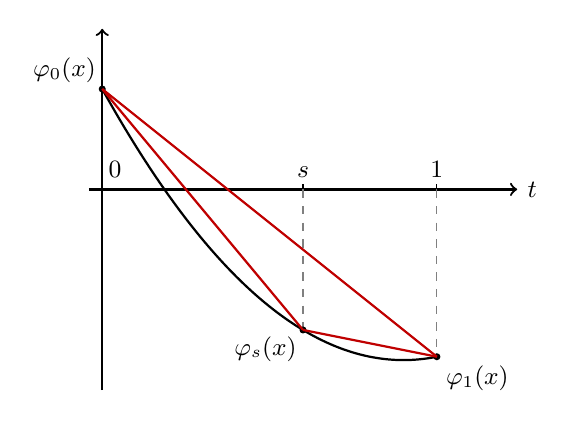
\begin{tikzpicture}[scale=0.85, line width=0.6pt, every node/.style={font=\small}]
  \draw[->, thick] (-0.2,0) -- (6.2,0) node[right] {$t$};
  \draw[->, thick] (0,-3.0) -- (0,2.4);
  % Ticks 0, s, 1 -- labels above the t-axis
  \draw[thin] (0,0.08) -- (0,-0.08);
  \draw[thin] (3,0.08) -- (3,-0.08);
  \draw[thin] (5,0.08) -- (5,-0.08);
  \node[anchor=south west, inner sep=2pt] at (0,0.08) {$0$};
  \node[anchor=south, inner sep=2pt] at (3,0.08) {$s$};
  \node[anchor=south, inner sep=2pt] at (5,0.08) {$1$};
  % Vertical dashed guides
  \draw[gray, dashed, thin] (3, 0) -- (3,-2.10);
  \draw[gray, dashed, thin] (5, 0) -- (5,-2.50);
  % Convex curve
  \draw[thick] plot[smooth, samples=80, domain=0:5] (\x, {1.5 - 1.8*\x + 0.20*\x*\x});
  \fill (0,1.5) circle (1.5pt);
  \fill (3,-2.10) circle (1.5pt);
  \fill (5,-2.50) circle (1.5pt);
  \node[anchor=south east, inner sep=2pt] at (0,1.5) {$\varphi_0(x)$};
  \node[anchor=north east, inner sep=2pt] at (3,-2.10) {$\varphi_s(x)$};
  \node[anchor=north west, inner sep=3pt] at (5,-2.50) {$\varphi_1(x)$};
  \draw[red!75!black, thick] (0,1.5) -- (3,-2.10);
  \draw[red!75!black, thick] (0,1.5) -- (5,-2.50);
  \draw[red!75!black, thick] (3,-2.10) -- (5,-2.50);
\end{tikzpicture}
\caption{Typical behaviour of $t\mapsto\varphi_t(x)$}
\label{fig:convphi}
\end{figure}
\begin{proof}
The notations in the proof are indicated in \cref{fig:convphi}.\footnote{When dealing with convex functions, drawing a picture is the easiest way to keep track of the directions of inequalities.}


    We may assume that $s\in (0,1)$ since there is nothing to prove when $s=0$ or $s=1$.

    After replacing $\varphi_t$ by $\varphi_t-C't$ for some large enough $C'>0$, we may assume that $\varphi_1\leq \varphi_0$. This procedure preserves the geodesic property by \cref{ex:lineargeod}. Then $\varphi_t$ is decreasing in $t$ by \cref{lma:geoddecreasing}.

    Let
    \begin{equation}\label{eq:Cdefsupvarphi1m0temp1}
        C=\sup_{\{\varphi_1\neq -\infty\}} \left(\varphi_1-\varphi_0\right)=\sup_{\{\varphi_0\neq -\infty\}} \left(\varphi_1-\varphi_0\right)\leq 0,
    \end{equation}
    where the equality is due to \cref{cor:diffsupinfindeppluripolar}.
    Then by \cref{prop:pshfuncdetdense}, we have
    \[
        \varphi_1\leq \varphi_0+C.
    \]
    So $(\varphi_1-C(1-t))_{t\in (0,1)}$ is a candidate in \eqref{eq:Perron2} and hence
    \begin{equation}\label{eq:varphi1leqvarphittemp}
        \varphi_1-C(1-t)\leq \varphi_t,\quad t\in (0,1).
    \end{equation}

    By \cref{prop:perronenvissubgeod}, we have $\varphi_t\xrightarrow{L^1}\varphi_1$ as $t\to 1-$.
    Since $\varphi_t$ is decreasing in $t\in (0,1)$, it follows that $\varphi_1=\inf_{t\in (0,1)}\varphi_t$.
    Therefore, we can find a pluripolar set $Z\subseteq X$ such that $\varphi_t(x)\rightarrow \varphi_1(x)>-\infty$ as $t\to 1-$ for all $x\in X\setminus Z$.

    Similarly, since $\varphi_0=\uscsup[t\in (0,1)] \varphi_t$, after enlarging $Z$, we may also guarantee that $\varphi_t(x)\rightarrow \varphi_0(x)>-\infty$ as $t\to 0+$ for all $x\in X\setminus Z$ by \cref{prop:supsupstardiff}.

    For any such $x\in X\setminus Z$, the function $t\mapsto \varphi_t(x)$ is a real-valued continuous convex function on $[0,1]$. In particular, $t\mapsto \varphi_t(x)$ is absolutely continuous on $[0,1]$.
    Hence, for any $s\in [0,1)$, we have
    \begin{equation}\label{eq:varphi1minusvarphi0temp1}
        \varphi_1(x)-\varphi_s(x)=\int_s^1 \ddt \varphi_t(x)\,\mathrm{d}t\leq (1-s)\lim_{t\to 1-}\frac{\varphi_1(x)-\varphi_t(x)}{1-t}\leq (1-s)C,
    \end{equation}
    where the second inequality follows from \eqref{eq:varphi1leqvarphittemp}.

    Taking supremum in \eqref{eq:varphi1minusvarphi0temp1}, we find that
    \begin{equation}\label{eq:supvarphi1sleqleqtemp1}
    \sup_{X\setminus Z} (\varphi_1-\varphi_s)\leq (1-s)\adjustlimits\sup_{x\in X\setminus Z}\lim_{t\to 1-}\frac{\varphi_1(x)-\varphi_t(x)}{1-t}\leq (1-s)C.
    \end{equation}
    When $s=0$, we deduce from \cref{cor:diffsupinfindeppluripolar} and \eqref{eq:Cdefsupvarphi1m0temp1} that
    \[
    C=\sup_{\{\varphi_1\neq -\infty\}} \left(\varphi_1-\varphi_0\right)=\adjustlimits\sup_{x\in X\setminus Z}\lim_{t\to 1-}\frac{\varphi_1(x)-\varphi_t(x)}{1-t}.
    \]
    But this equality works equally well for the geodesic $(\varphi_{(1-s)t+s})_{t\in [0,1]}$ with the same argument. It follows that
    \[
    \sup_{\{\varphi_1\neq -\infty\}} \left(\varphi_1-\varphi_s\right)=(1-s)\adjustlimits\sup_{x\in X\setminus Z}\lim_{t\to 1-}\frac{\varphi_1(x)-\varphi_t(x)}{1-t}=(1-s)C.
    \]
    Therefore, invoking \cref{cor:diffsupinfindeppluripolar} again, we deduce that all inequalities in \eqref{eq:supvarphi1sleqleqtemp1} are in fact equalities. In other words,
    \begin{equation}\label{eq:supvarphi1mivarphi0temp1}
        \sup_{\{\varphi_1\neq -\infty\}}(\varphi_1-\varphi_0)=   \adjustlimits \sup_{x\in X\setminus Z}\lim_{t\to 1-}\frac{\varphi_1(x)-\varphi_t(x)}{1-t}
        =\sup_{\{\varphi_1\neq -\infty\}}\frac{\varphi_1-\varphi_s}{1-s}.
    \end{equation}
    On the other hand, we have the trivial inequality when $s\in (0,1)$:
    \[
    \sup_{\{\varphi_1\neq -\infty\}}(\varphi_1-\varphi_0)\leq s \sup_{\{\varphi_1\neq -\infty\}}\frac{\varphi_s-\varphi_0}{s}+   (1-s) \sup_{\{\varphi_1\neq -\infty\}}\frac{\varphi_1-\varphi_s}{1-s}.
    \]
    Together with \eqref{eq:supvarphi1mivarphi0temp1}, we find that for $s\in (0,1)$,
    \[
    \sup_{\{\varphi_1\neq -\infty\}}(\varphi_1-\varphi_0)\leq \sup_{\{\varphi_1\neq -\infty\}}\frac{\varphi_s-\varphi_0}{s}.
    \]
    The reverse inequality follows from the convexity, and hence for $s\in (0,1)$, we have
    \[
        \sup_{\{\varphi_1\neq -\infty\}}\frac{\varphi_s-\varphi_0}{s}=\sup_{\{\varphi_1\neq -\infty\}}(\varphi_1-\varphi_0).
    \]
    Using \cref{cor:diffsupinfindeppluripolar}, we conclude \eqref{eq:tsupsuptemp1}.
\end{proof}

With an almost identical proof, we find
\begin{proposition}\label{prop:geodinfsublinear}
    Let $\varphi_1,\varphi_0\in \mathcal{E}^{\infty}(X,\theta;\phi)$. Let $(\varphi_t)_{t\in (0,1)}$ be the geodesic from $\varphi_0$ to $\varphi_1$. Then
    \[
        t\inf_{\{\phi\neq -\infty\}}(\varphi_1-\varphi_0)=\inf_{\{\phi\neq -\infty\}}(\varphi_t-\varphi_0)
    \]
    for all $t\in (0,1]$.
\end{proposition}

\begin{definition}\label{def:geodraydef}
    Let $\ell=(\ell_t)_{t\geq 0}$ be a family in $\mathcal{E}(X,\theta;\phi)$. We say $\ell$ is a \emph{geodesic ray}\index{geodesic ray} in $\mathcal{E}(X,\theta;\phi)$ emanating from $\ell_0$ if for each $0\leq a\leq b$, the restriction $(\ell_t)_{t\in [a,b]}$ is a geodesic.

    The set of geodesic rays in $\mathcal{E}(X,\theta;\phi)$ emanating from $\phi$ is denoted by $\mathcal{R}(X,\theta;\phi)$\index{$\mathcal{R}(X,\theta;\phi)$}.

    We say a geodesic ray $\ell\in \mathcal{R}(X,\theta;\phi)$ has \emph{finite energy}\index{geodesic ray!geodesic ray with finite energy} if $\ell_t\in \mathcal{E}^1(X,\theta;\phi)$ for all $t>0$. The set of geodesic rays with finite energy is denoted by $\mathcal{R}^1(X,\theta;\phi)$\index{$\mathcal{R}^1(X,\theta;\phi)$}.

    We say a geodesic ray $\ell\in \mathcal{R}(X,\theta;\phi)$ is \emph{bounded}\index{geodesic ray!bounded geodesic ray} if $\ell_t\in \mathcal{E}^{\infty}(X,\theta;\phi)$ for all $t\geq 0$. The set of bounded geodesic rays is denoted by $\mathcal{R}^{\infty}(X,\theta;\phi)$\index{$\mathcal{R}^{\infty}(X,\theta;\phi)$}.

    Given $\ell,\ell'\in \mathcal{R}(X,\theta;\phi)$, we write $\ell\leq \ell'$ if $\ell_t\leq \ell'_t$ for each $t\geq 0$.

    When $\phi=V_{\theta}$, we usually omit it from the notations and write $\mathcal{R}(X,\theta)$\index{$\mathcal{R}(X,\theta)$}, $\mathcal{R}^1(X,\theta)$\index{$\mathcal{R}^1(X,\theta)$} and $\mathcal{R}^{\infty}(X,\theta)$\index{$\mathcal{R}^{\infty}(X,\theta)$} respectively.
\end{definition}

\begin{proposition}\label{prop:raysuplinear}
    Let $\ell\in \mathcal{R}(X,\theta;\phi)$. Then there is a constant $C\in \mathbb{R}$ such that
    \[
        \sup_{X}\ell_t=Ct,\quad t\geq 0.
    \]
\end{proposition}
\begin{proof}
    It follows from \cref{prop:geodsupsublinear} that
    \[
    \sup_{\{\phi\neq -\infty\}}(\ell_t-\phi)=t\sup_{\{\phi\neq -\infty\}}(\ell_1-\phi)
    \]
    for all $t\geq 0$.

    It suffices to show that for any $t\geq 0$,
    \[
    \sup_{\{\phi\neq -\infty\}}(\ell_t-\phi)=\sup_X \ell_t.
    \]
    This was already proved in \cref{prop:model_sup_prop}.
\end{proof}





\section{The metrics on the spaces of potentials and rays}\label{sec:metE1}

Let $X$ be a connected compact Kähler manifold of dimension $n$ and $\theta$ be a smooth closed real $(1,1)$-form on $X$ representing a big cohomology class.
Fix a model potential $\phi\in \PSH(X,\theta)_{>0}$.

We first study a natural metric on $\mathcal{E}^1(X,\theta;\phi)$.

\begin{definition}\label{def:d1onE12}
    Let $\varphi,\psi\in \mathcal{E}^1(X,\theta;\phi)$, we define the \emph{Darvas metric}\index{Darvas metric} $d_1$ as follows:
    \[
        d_1(\varphi,\psi)=E_{\theta}^{\phi}(\varphi)+E_{\theta}^{\phi}(\psi)-2E_{\theta}^{\phi}(\varphi\land \psi).
    \]
    Note that by \cref{prop:relrooftopclosed}, $\varphi\land \psi\in \mathcal{E}^1(X,\theta;\phi)$.
\end{definition}
Recall that $E_{\theta}^{\phi}$ is defined in \cref{def:MAenergy}.

In particular, if $\varphi\leq \psi$, we have
\begin{equation}\label{eq:d1asEdiff}
    d_1(\varphi,\psi)=E_{\theta}^{\phi}(\psi)-E_{\theta}^{\phi}(\varphi).
\end{equation}

We wish to show that $d_1$ is a complete metric. We first prove a contraction property:
\begin{proposition}\label{prop:d1contract}
    Let $\varphi,\psi,\gamma\in \mathcal{E}^1(X,\theta;\phi)$. Then
    \begin{equation}\label{eq:d1contract}
    d_1(\varphi,\psi)\geq d_1(\varphi\land \gamma,\psi\land \gamma).
    \end{equation}
\end{proposition}
\begin{proof}
    \textbf{Step~1}. We first assume that $\varphi\geq \psi$. Then
    \[
    \begin{aligned}
        d_1(\varphi,\psi)=& E_{\theta}^{\phi}(\varphi)-E_{\theta}^{\phi}(\psi)\\
        \geq & E_{\theta}^{\phi}\Bigl((\varphi\land \gamma)\lor \psi\Bigr)-E_{\theta}^{\phi}(\psi) & \textup{by \cref{lma:EmonoEinfty}}\\
        \geq & E_{\theta}^{\phi}(\varphi\land \gamma)-E_{\theta}^{\phi}(\psi\land \gamma)&\textup{by \cref{cor:diam_E}}.
    \end{aligned}
    \]

    \textbf{Step~2}. We prove the general case.

    By Step~1, we have
    \[
    d_1(\varphi,\varphi\land \psi)\geq d_1(\varphi\land \gamma,\varphi\land \psi\land \gamma),\quad d_1(\psi,\varphi\land \psi)\geq d_1(\psi\land \gamma,\varphi\land \psi\land \gamma).
    \]
    Adding the two inequalities together, we conclude \eqref{eq:d1contract}.
\end{proof}


\begin{lemma}\label{lma:d1metric}
    The function $d_1$ is a metric on $\mathcal{E}^1(X,\theta;\phi)$.
\end{lemma}
\begin{proof}
    There are two facts to prove, as in the two steps below.

    \textbf{Step~1}. Let $\varphi,\psi\in \mathcal{E}^1(X,\theta;\phi)$. Assume that $d_1(\varphi,\psi)=0$. Then we will show that $\varphi=\psi$.

    We first treat the case $\psi\leq \varphi$. Then $d_1(\varphi,\psi)=E_\theta^\phi(\varphi)-E_\theta^\phi(\psi)=0$, and \cref{prop:cocycE1} gives
    \[
    \int_X (\varphi-\psi)\,\theta_{\psi}^n=0.
    \]
    We conclude that $\psi=\varphi$ using the domination principle \cref{thm:dom_prin_1}.

    In general, put $\gamma=\varphi\land\psi$. Since
    \[
    d_1(\varphi,\psi)=d_1(\varphi,\gamma)+d_1(\psi,\gamma),
    \]
    both terms on the right vanish. Applying the comparable case to the pairs $(\varphi,\gamma)$ and $(\psi,\gamma)$ gives $\varphi=\gamma=\psi$.

    \textbf{Step~2}. Let $\varphi,\psi,\gamma\in \mathcal{E}^1(X,\theta;\phi)$. We prove the triangle inequality:
    \[
    d_1(\varphi,\psi)\leq d_1(\varphi,\gamma)+d_1(\psi,\gamma).
    \]
    This can be translated to
    \[
    E_{\theta}^{\phi}(\varphi\land \gamma)-E_{\theta}^{\phi}(\varphi\land \psi)\leq E_{\theta}^{\phi}(\gamma)-E_{\theta}^{\phi}(\psi\land \gamma).
    \]
    We just have to compute using \cref{prop:d1contract}:
    \[
    \begin{aligned}
        E_{\theta}^{\phi}(\gamma)-E_{\theta}^{\phi}(\psi\land \gamma)\geq & E_{\theta}^{\phi}(\varphi\land \gamma)-E_{\theta}^{\phi}(\varphi\land \psi\land \gamma)\\
        \geq &E_{\theta}^{\phi}(\varphi\land \gamma)-E_{\theta}^{\phi}(\varphi\land \psi),
    \end{aligned}
    \]
    where the second line follows from \cref{lma:EmonoEinfty}.
\end{proof}


We introduce an auxiliary functional.
\begin{definition}\label{def:Itheta}
    Define $I_{\theta}\colon \mathcal{E}^1(X,\theta;\phi)\times \mathcal{E}^1(X,\theta;\phi)\rightarrow \mathbb{R}\cup \{\infty\}$ as follows:
    \begin{equation}
        I_{\theta}(\varphi,\psi)\coloneqq \int_X |\varphi-\psi|\left( \theta_{\varphi}^n+\theta_{\psi}^n \right).
    \end{equation}
    \index{$I_{\theta}$}
\end{definition}
We will soon see that $I_{\theta}$ is always finite, see \cref{thm:I_d1_comp}.

We observe the following elementary equality.
\begin{lemma}\label{lma:I_equal_Imaxsum}
    Let $\varphi,\psi\in \mathcal{E}^1(X,\theta;\phi)$. Then
    \[
    I_{\theta}(\varphi,\psi)=I_{\theta}(\varphi\lor \psi,\varphi)+I_{\theta}(\varphi\lor \psi,\psi).
    \]
\end{lemma}
\begin{proof}
    By the plurifine locality of non-pluripolar products \itemref{itm:prop:npp1:1}, we can write
    \[
    \begin{aligned}
         I_{\theta}(\varphi,\psi)=&\int_{ \{\varphi<\psi\}} (\psi-\varphi) \left( \theta_{\varphi}^n+\theta_{\psi}^n \right)+\int_{ \{\varphi>\psi\}} (\varphi-\psi) \left( \theta_{\varphi}^n+\theta_{\psi}^n \right),\\
         I_{\theta}(\varphi\lor \psi,\varphi)=& \int_{\{\psi>\varphi\}} (\psi-\varphi)\left(\theta_{\psi}^n+\theta_{\varphi}^n \right),\\
         I_{\theta}(\varphi\lor \psi,\psi)=& \int_{\{\psi<\varphi\}} (\varphi-\psi)\left(\theta_{\psi}^n+\theta_{\varphi}^n \right).
    \end{aligned}
    \]
    The desired equality follows by comparing these terms.
\end{proof}

We have an interesting relation between $d_1$ and $I_{\theta}$ defined in \cref{def:Itheta}.
\begin{theorem}\label{thm:I_d1_comp}
    Let $\varphi,\psi\in \mathcal{E}^1(X,\theta;\phi)$. Then
    \begin{equation}\label{eq:I_d1_comp}
    \frac{1}{C_n} I_{\theta}(\varphi,\psi)\leq d_1(\varphi,\psi)\leq I_{\theta}(\varphi,\psi),
    \end{equation}
    where $C_n=3\cdot 2^{n+2}(n+1)$.
\end{theorem}
\begin{proof}
    \textbf{Step~1}. We first prove the right-hand part of \eqref{eq:I_d1_comp}.

    Thanks to \cref{prop:Ediffbdd} and \cref{lma:rooftopMA}, we have
    \[
    \begin{aligned}
    E_{\theta}^{\phi}(\varphi)-E_{\theta}^{\phi}(\varphi\land \psi)\leq & \int_X (\varphi-\varphi\land\psi)\,\theta_{\varphi\land \psi}^n \\
    \leq & \int_{\{\psi=\varphi\land \psi \}} (\varphi-\psi)\,\theta_{\psi}^n\\
    \leq & \int_X |\varphi-\psi|\,\theta_{\psi}^n.
    \end{aligned}
    \]
    Similarly,
    \[
    E_{\theta}^{\phi}(\psi)-E_{\theta}^{\phi}(\varphi\land \psi)\leq \int_X |\varphi-\psi|\,\theta_{\varphi}^n.
    \]
    Adding these inequalities up, we find
    \[
    d_1(\varphi,\psi)\leq I_{\theta}(\varphi,\psi).
    \]

    \textbf{Step~2}. We prove the left-hand part of \eqref{eq:I_d1_comp}.

    We claim that
    \begin{equation}\label{eq:d_1varphivarphipsimean_temp1}
        d_1\left(\varphi,\frac{\varphi+\psi}{2}\right)\leq \frac{3(n+1)}{2} d_1(\varphi,\psi).
    \end{equation}
    For this purpose, we compute directly
    \[
    \begin{aligned}
        &d_1\left(\varphi,\frac{\varphi+\psi}{2}\right)\\
        =&d_1\left(\varphi,\varphi\land \frac{\varphi+\psi}{2}\right)+d_1\left(\frac{\varphi+\psi}{2},\varphi\land \frac{\varphi+\psi}{2}\right)\\
        \leq & d_1\left(\varphi,\varphi\land \psi\right)+d_1\left(\frac{\varphi+\psi}{2},\varphi\land\psi\right)&\textup{by \cref{lma:EmonoEinfty}}\\
        \leq & \int_X \left( \varphi-\varphi\land\psi\right)\,\theta_{\varphi\land\psi}^n+ \int_X \left( \frac{\varphi+\psi}{2}-\varphi\land\psi\right)\,\theta_{\varphi\land \psi}^n &\textup{by \cref{prop:Ediffbdd}}\\
        =& \frac{3}{2}\int_X \left( \varphi-\varphi\land\psi\right)\,\theta_{\varphi\land\psi}^n+\frac{1}{2}\int_X \left( \psi-\varphi\land\psi\right)\,\theta_{\varphi\land\psi}^n \\
        \leq & \frac{3(n+1)}{2}d_1\left(\varphi,\varphi\land \psi\right) + \frac{n+1}{2}d_1(\psi,\varphi\land \psi)& \textup{by \eqref{eq:Ecocyc}}\\
        \leq & \frac{3(n+1)}{2}d_1(\varphi,\psi),
    \end{aligned}
    \]
    and \eqref{eq:d_1varphivarphipsimean_temp1} follows.

    We now estimate the left-hand side of \eqref{eq:d_1varphivarphipsimean_temp1}:
    \[
    \begin{aligned}
    d_1\left(\varphi,\frac{\varphi+\psi}{2}\right)\geq & d_1\left(\varphi,\varphi\land \frac{\varphi+\psi}{2}\right)\\
    \geq & \int_X \left(\varphi-\varphi\land \frac{\varphi+\psi}{2}\right)\,\theta_{\varphi}^n\\
    \geq & \int_{\{\varphi>\psi\}}\left(\varphi-\varphi\land \frac{\varphi+\psi}{2}\right)\,\theta_{\varphi}^n \\
    \geq & \int_{\{\varphi>\psi\}}\left(\varphi-\frac{\varphi+\psi}{2}\right)\,\theta_{\varphi}^n\\
    =& \frac{1}{2}\int_{\{\varphi>\psi\}}\left(\varphi-\psi\right)\,\theta_{\varphi}^n,
    \end{aligned}
    \]
    where the second inequality follows from \cref{prop:Ediffbdd}.

    Similarly,
    \[
    \begin{aligned}
        d_1\left(\varphi,\frac{\varphi+\psi}{2}\right)\geq & d_1\left(\frac{\varphi+\psi}{2},\varphi\land \frac{\varphi+\psi}{2}\right)\\
        \geq & \int_X \left(\frac{\varphi+\psi}{2}-\varphi\land \frac{\varphi+\psi}{2}\right)\,\theta_{(\varphi+\psi)/2}^n\\
        \geq & 2^{-n} \int_X \left(\frac{\varphi+\psi}{2}-\varphi\land \frac{\varphi+\psi}{2}\right)\,\theta_{\varphi}^n\\
        \geq & 2^{-n} \int_{\{\varphi<\psi\}} \left(\frac{\varphi+\psi}{2}-\varphi\land \frac{\varphi+\psi}{2}\right)\,\theta_{\varphi}^n\\
        \geq & 2^{-n} \int_{\{\varphi<\psi\}} \left(\frac{\varphi+\psi}{2}-\varphi\right)\,\theta_{\varphi}^n\\
        =& 2^{-n-1} \int_{\{\varphi<\psi\}} \left(\psi-\varphi\right)\,\theta_{\varphi}^n,
    \end{aligned}
    \]
    where the third inequality follows from the multi-linearity of the non-pluripolar product \itemref{itm:prop:npp1:6}.


    Adding these estimates up, we find
    \[
        2^{n+2} d_1\left(\varphi,\frac{\varphi+\psi}{2}\right)\geq \left(2^{n+1}+2\right) d_1\left(\varphi,\frac{\varphi+\psi}{2}\right)\geq \int_X |\varphi-\psi|\,\theta_{\varphi}^n.
    \]
    Therefore, combined with \eqref{eq:d_1varphivarphipsimean_temp1} we conclude
    \[
    3\cdot 2^{n+1}(n+1)d_1(\varphi,\psi)\geq \int_X |\varphi-\psi|\,\theta_{\varphi}^n.
    \]
    By symmetry, we also get a similar expression after exchanging $\varphi$ and $\psi$. Adding these inequalities together, we find
    \[
    3\cdot 2^{n+2}(n+1)d_1(\varphi,\psi)\geq I_{\theta}(\varphi,\psi).
    \]
    The left-hand part of \eqref{eq:I_d1_comp} then follows.
\end{proof}

\begin{corollary}\label{cor:d1maxonearg}
    Let $\varphi,\psi\in \mathcal{E}^1(X,\theta;\phi)$. Then
    \begin{equation}\label{eq:d1maxonearg}
        d_1(\varphi\lor \psi,\varphi)\leq C_n d_1(\varphi,\psi),
    \end{equation}
    where $C_n$ is the constant in \cref{thm:I_d1_comp}.
\end{corollary}
\begin{proof}
    By \cref{thm:I_d1_comp} and \cref{lma:I_equal_Imaxsum}, we have
    \[
        d_1(\varphi\lor\psi,\varphi)\leq I_{\theta}(\varphi\lor\psi,\varphi)\leq I_{\theta}(\varphi,\psi)\leq C_n d_1(\varphi,\psi).
    \]
    This completes the proof.
\end{proof}

\begin{lemma}\label{lma:d1bdsupX}
    There is $A,B>0$ so that for any $\varphi\in \mathcal{E}^1(X,\theta;\phi)$,  we have
    \begin{equation}\label{eq:d1bdsupX}
    d_1(\varphi,\phi)\geq -\int_X \theta_{\phi}^n\cdot \sup_X \varphi\geq -Ad_1(\varphi,\phi)-B.
    \end{equation}
\end{lemma}
\begin{proof}
    When $\sup_X \varphi\leq 0$, the right-hand part of \eqref{eq:d1bdsupX} is trivial. Since $\varphi\leq \phi$, we find
    \[
    d_1(\phi,\varphi)=-E_{\theta}^{\phi}(\varphi)\geq -\int_X \theta_{\phi}^n\cdot\sup_{\{\phi\neq -\infty\}} (\varphi-\phi)=-\int_X \theta_{\phi}^n\cdot\sup_X \varphi,
    \]
    where the last equality follows from \cref{prop:model_sup_prop}.

    We can therefore assume that $\sup_X \varphi> 0$. In this case, the left-hand part of \eqref{eq:d1bdsupX} is trivial. Take a Kähler form $\omega\geq \theta$ on $X$. Then thanks to \cref{thm:Pvarphisupport}, we can find a constant $C>0$ so that
    \[
    \theta_{\phi}^n\leq C\omega^n.
    \]
    Thanks to \cref{prop:L1compa}, there is a constant $C'>0$, independent of the choice of $\varphi$, so that
    \[
    \int_X \left( \phi-\varphi+\sup_X \varphi \right)\,\theta_{\phi}^n\leq C'.
    \]
    We estimate
    \[
    \begin{aligned}
    I_{\theta}(\phi,\varphi)\geq & \int_X |\varphi-\phi|\,\theta_{\phi}^n\\
    \geq & \left(\sup_X \varphi\right)\int_X \theta_{\phi}^n-\int_X \left( \phi-\varphi+\sup_X \varphi \right)\,\theta_{\phi}^n \\
    \geq & \left(\sup_X \varphi\right)\int_X \theta_{\phi}^n-C'.
    \end{aligned}
    \]
    The right-hand part of \eqref{eq:d1bdsupX} then follows from \cref{thm:I_d1_comp}.
\end{proof}

Next we handle the completeness of $d_1$. The completeness can be proved in a more general framework.
\begin{definition}\label{def:rays:L858}
	Let $E$ be a set. A \emph{pre-rooftop structure} on $E$ is a binary operator $\land:E\times E\rightarrow E$, satisfying the following axioms: For $x,y,z\in E$,
	\begin{enumerate}
		\item\label{itm:chapter-rays:L841:1} $x\land y=y\land x$.
		\item\label{itm:chapter-rays:L841:2} $(x\land y)\land z=x\land (y\land z)$.
		\item\label{itm:chapter-rays:L841:3} $x\land x=x$.
	\end{enumerate}
	We call $(E,\land)$ a \emph{pre-rooftop space}\index{pre-rooftop space}.
\end{definition}

A pre-rooftop structure $\land$ defines a partial order $\leq$ on $E$ as follows:
\[
x\leq y\quad \text{if and only if } \quad x\land y=x.
\]
Here by abuse of notation, we use $\leq$ to denote the partial order.

In particular, it makes sense to talk about increasing and decreasing sequences in $E$.

\begin{definition}\label{def:roof}
	Let $(E,d)$ be a metric space. A \emph{pre-rooftop structure}\index{pre-rooftop structure} on $(E,d)$ is a pre-rooftop structure $\land$ on $E$. We say $(E,d,\land)$ is a \emph{pre-rooftop metric space}\index{pre-rooftop metric space}.

	A \emph{rooftop structure}\index{rooftop structure} on $(E,d)$ is a pre-rooftop structure $\land$ on $E$ such that
	\begin{equation}\label{eq:rtdef}
		d(x\land z,y\land z)\leq d(x,y),\quad \forall x,y,z\in E.
	\end{equation}
	We call $(E,d,\land)$ a \emph{rooftop metric space}\index{rooftop metric space}.
\end{definition}

\begin{lemma}\label{lma:landdis}
	Let $(E,d,\land)$ be a rooftop metric space. Let $x,y,x',y'\in E$. Then
	\begin{equation}
		d(x\land y,x'\land y')\leq d(x,x')+d(y,y').
	\end{equation}
\end{lemma}
In particular, $\land\colon E\times E\rightarrow E$ is continuous.
\begin{proof}
	We compute
	\[
	d(x\land y,x'\land y')\leq d(x\land y,x\land y')+d(x\land y',x'\land y')\leq d(x,x')+d(y,y').
	\]
	This completes the proof.
\end{proof}

\begin{proposition}\label{prop:rooftopcomp}
	Let $(E,d,\land)$ be a rooftop metric space. Then $(E,d)$ is complete if and only if both of the following hold:
	\begin{enumerate}
		\item\label{itm:prop:rooftopcomp:1} Each increasing Cauchy sequence converges.
		\item\label{itm:prop:rooftopcomp:2} Each decreasing Cauchy sequence converges.
	\end{enumerate}
\end{proposition}
\begin{proof}
	The direct implication is trivial.

	Conversely, assume that both conditions are true.
	Let $(x_j)_{j>0}$ be a Cauchy sequence in $E$. We want to prove that $(x_j)_j$ converges. By passing to a subsequence, we may assume that
	\[
	d\left(x_j,x_{j+1}\right)\leq 2^{-j}.
	\]
	For $k,j\geq 1$, let
	\[
	y_j^k\coloneqq x_k\land \cdots \land x_{k+j}.
	\]
	Then $(y_j^k)_j$ is decreasing, and
	\[
	d\left(y_j^k,y_{j+1}^k\right)\leq d\left(x_{k+j},x_{k+j+1}\right)\leq 2^{-k-j}.
	\]
	So $(y_j^k)_j$ is a decreasing Cauchy sequence. Define
	\[
	y^k\coloneqq \lim_{j\to\infty}y_j^k.
	\]
	Then
	\[
	d\left(y^k,y^{k+1}\right)=\lim_{j\to\infty}d\left(y_{j+1}^k,y_j^{k+1}\right)\leq d\left(x_k,x_{k+1}\right)\leq 2^{-k}.
	\]
    We also need to check that the sequence $(y^k)_k$ is increasing. For each $j\geq 1$, we have
    \[
        y_j^k=x_k\land y_{j-1}^{k+1}\leq y_{j-1}^{k+1}.
    \]
    Equivalently,
    \[
        y_j^k\land y_{j-1}^{k+1}=y_j^k.
    \]
    Letting $j\to\infty$ and using the continuity of $\land$ from \cref{lma:landdis}, we obtain
    \[
        y^k\land y^{k+1}=y^k.
    \]
    Thus $y^k\leq y^{k+1}$.
	So $(y^k)_k$ is an increasing Cauchy sequence. Let
	\[
	y\coloneqq \lim_{k\to\infty}y^k.
	\]
	For every $j\geq 0$, we have
	\[
	    d\left(y_j^k,x_k\right)\leq \sum_{r=k}^{k+j-1}d\left(x_r,x_{r+1}\right),
	\]
	with the empty sum understood as $0$. Indeed, this is trivial for $j=0$, and the induction step follows from
	\[
	    y_j^k=x_k\land y_{j-1}^{k+1}
	\]
	and
	\[
	    d\left(y_j^k,x_k\right)\leq d\left(y_{j-1}^{k+1},x_k\right)\leq d\left(y_{j-1}^{k+1},x_{k+1}\right)+d\left(x_{k+1},x_k\right).
	\]
	Letting $j\to\infty$, we get
	\[
	d\left(y^k,x_k\right)\leq \sum_{r=k}^{\infty}d\left(x_r,x_{r+1}\right)\leq 2^{1-k}.
	\]
	So $(x_k)_k$ converges to $y$.
\end{proof}


\begin{theorem}\label{thm:d1_complete}
    The metric space $(\mathcal{E}^1(X,\theta;\phi),d_1)$ is complete.
\end{theorem}
It follows from the proof below that if $(\varphi_j)_{j>0}$ is a monotone sequence in $\mathcal{E}^1(X,\theta;\phi)$ with $d_1$-limit $\varphi$, then $\varphi$ is the almost everywhere limit of $(\varphi_j)_{j>0}$. We will use this result without further explanation in the sequel.
\begin{proof}
    As we have seen in \cref{lma:d1metric} and \cref{prop:d1contract}, the triple
    \[
    \left(\mathcal{E}^1(X,\theta;\phi),d_1,\land \right)
    \]
    is a rooftop metric space. Hence thanks to \cref{prop:rooftopcomp}, it remains to show that each increasing or decreasing Cauchy sequence in $\mathcal{E}^1(X,\theta;\phi)$ converges.

    We first consider an increasing sequence $(\varphi_i)_{i>0}$ in $\mathcal{E}^1(X,\theta;\phi)$. The Cauchy property simply means that
    \[
    \sup_{i>0} E_{\theta}^{\phi}(\varphi_i)<\infty.
    \]
    We claim that
    \[
    \varphi\coloneqq \uscsup[i>0]\varphi_i
    \]
    is the $d_1$-limit of the sequence. We first observe that $(\sup_X \varphi_i)_{i>0}$ is bounded, as a consequence of \cref{lma:d1bdsupX}. Therefore, \cref{prop:supsEE1} guarantees that $\varphi\in \mathcal{E}^1(X,\theta;\phi)$, and hence our assertion follows from \cref{prop:Econt_mono}.

    Next we consider a decreasing sequence $(\varphi_i)_{i>0}$ in $\mathcal{E}^1(X,\theta;\phi)$. The Cauchy property simply means that
    \[
    \inf_{i>0} E_{\theta}^{\phi}(\varphi_i)>-\infty.
    \]
    We claim that
    \[
     \varphi\coloneqq \inf_{i>0}\varphi_i
    \]
    is the $d_1$-limit of the sequence. Equivalently, we need to show that $\varphi\in \mathcal{E}^1(X,\theta;\phi)$ and
    \begin{equation}\label{eq:E_cont_decnet_temp1}
        E_{\theta}^{\phi}(\varphi)=\lim_{i\to\infty} E_{\theta}^{\phi}(\varphi_i).
    \end{equation}

    We first observe that $(\sup_X \varphi_i)_{i>0}$ is bounded, as a consequence of \cref{lma:d1bdsupX}. Therefore, $\varphi\in \PSH(X,\theta;\phi)$ and $\varphi_i\xlongrightarrow{L^1} \varphi$, see \cref{cor:decreasingnetL1conv}. We claim that $\varphi\in \mathcal{E}^1(X,\theta;\phi)$. For this purpose, we may assume that $\varphi_1\leq 0$.
    Since $(\varphi_i)_i$ is decreasing, $\varphi_i\leq \varphi_1\leq 0$ for all $i>0$. As $\varphi_i\preceq\phi$ and $\phi$ is model, each $\varphi_i$ is a candidate for $P_\theta[\phi]=\phi$, so $\varphi_i\leq \phi$. Thus, using the energy formula \eqref{eq:Edefbdd} and the fact that all mixed terms are non-positive, we get for each $i>0$,
    \[
        \frac{1}{n+1}\int_X \left(\varphi_i-\phi\right)\,\theta_{\varphi_i}^n\geq E_{\theta}^{\phi}(\varphi_i)\geq \inf_{j>0} E_{\theta}^{\phi}(\varphi_j)>-\infty.
    \]
    We can then apply \cref{lma:stab}, with $\gamma=\phi$, to conclude that $\varphi\in \mathcal{E}^1(X,\theta;\phi)$.
    Our assertion \eqref{eq:E_cont_decnet_temp1} then follows from \cref{prop:E_cont_decnet}. We conclude the proof.
\end{proof}

\begin{lemma}\label{lma:d1conv_inbetween_mono}
    Let $(\varphi_i)_{i>0}$ be a sequence in $\mathcal{E}^1(X,\theta;\phi)$ with $d_1$-limit $\varphi\in \mathcal{E}^1(X,\theta;\phi)$. Then after replacing $(\varphi_i)_{i>0}$ by a subsequence, we can find two sequences $(\psi_i)_{i>0}$ and $(\eta_i)_{i>0}$ in $\mathcal{E}^1(X,\theta;\phi)$ such that
    \begin{enumerate}
        \item\label{itm:lma:d1conv_inbetween_mono:1} $(\psi_i)_{i>0}$ is decreasing with $d_1$ and pointwise limit $\varphi$;
        \item\label{itm:lma:d1conv_inbetween_mono:2} $(\eta_i)_{i>0}$ is increasing with $d_1$ and almost everywhere limit $\varphi$.
        \item\label{itm:lma:d1conv_inbetween_mono:3} $\eta_i\leq \varphi_i\leq \psi_i$ for all $i>0$.
    \end{enumerate}
\end{lemma}
\begin{proof}
    We first note that as a consequence of \cref{lma:d1bdsupX}, $(\sup_X \varphi_i)_{i>0}$ is bounded.
    Let $C_n$ be the constant in \cref{thm:I_d1_comp}. After replacing $(\varphi_i)_{i>0}$ by a subsequence, we may assume that
    \[
    d_1(\varphi_i,\varphi_{i+1})\leq \min\{C_n^{-2i},2^{-i}\}.
    \]

    We first construct $(\psi_i)_{i>0}$. For this purpose, it suffices to define
    \[
    \psi_i\coloneqq \uscsup[j\geq i] \varphi_j
    \]
    for each $i>0$.
    It follows from \cref{prop:supsEE1} that $\psi_i\in \mathcal{E}^1(X,\theta;\phi)$ for each $i>0$.
    For $k\geq 0$, set
    \[
        \psi_i^k\coloneqq \varphi_i\lor\varphi_{i+1}\lor\cdots\lor\varphi_{i+k}.
    \]
    Iterating \cref{cor:d1maxonearg} gives
    \[
    d_1(\varphi_i,\psi_i^k)\leq \sum_{a=i}^{i+k-1}C_n^{a+1-i}d_1(\varphi_a,\varphi_{a+1})\leq \sum_{a=i}^{i+k-1}C_n^{a+1-i}C_n^{-2a}.
    \]
    Since $\psi_i^k$ increases almost everywhere to $\psi_i$, letting $k\to\infty$ and using \cref{prop:Econt_mono}, we get
    \[
        d_1(\varphi_i,\psi_i)\leq \frac{C_n^{1-2i}}{1-C_n^{-1}}.
    \]
    Thus $\psi_i\to\varphi$ in $d_1$. Since $(\psi_i)_i$ is decreasing, the monotone case in the proof of \cref{thm:d1_complete} shows that $\psi_i$ converges almost everywhere to $\varphi$, hence pointwise by \cref{prop:pshfuncdetdense}.

    Next we construct $(\eta_i)_{i>0}$.
    For each $i>0$ and $k\geq 0$, we let
    \[
    \eta_i^k\coloneqq \varphi_i\land \varphi_{i+1}\land \cdots\land \varphi_{i+k}.
    \]
    Then
    \[
    \begin{aligned}
    d_1(\varphi_i,\eta_i^k)\leq & \sum_{j=0}^{k-1} d_1\left(\eta_i^j,\eta_i^{j+1}\right)\\
    \leq &\sum_{j=0}^{k-1} d_1\left(\varphi_{i+j},\varphi_{i+j+1}\right) &\textup{by \cref{prop:d1contract}}\\
    \leq & \sum_{j=0}^{k-1} 2^{-i-j}\\
    \leq & 2^{1-i}.
    \end{aligned}
    \]
    Since $\eta_i^k\leq \varphi_i$, the preceding estimate gives
    \[
        E_{\theta}^{\phi}(\eta_i^k)\geq E_{\theta}^{\phi}(\varphi_i)-2^{1-i},\quad k\geq 0.
    \]
    The sequence $(\eta_i^k)_{k\geq 0}$ is decreasing, and the monotonicity of $E_{\theta}^{\phi}$ shows that the sequence $\left(E_{\theta}^{\phi}(\eta_i^k)\right)_{k\geq 0}$ is decreasing and bounded from below, hence convergent. Thus, for $k\leq l$,
    \[
        d_1(\eta_i^k,\eta_i^l)=E_{\theta}^{\phi}(\eta_i^k)-E_{\theta}^{\phi}(\eta_i^l),
    \]
    and $(\eta_i^k)_{k\geq 0}$ is a decreasing Cauchy sequence. Therefore, the monotone case in the proof of \cref{thm:d1_complete} shows that
    \[
    \eta_i\coloneqq \lim_{k\to\infty}\eta_i^k=\inf_{k\geq 0} \eta_i^k
    \]
    is the $d_1$-limit of $(\eta_i^k)_{k\geq 0}$ and \cref{prop:Econt_mono} shows that
    \[
    d_1(\varphi_i,\eta_i)\leq 2^{1-i}.
    \]
    By construction, $\eta_i\leq \varphi_i$ and $(\eta_i)_i$ is increasing. Therefore, $\varphi$ is the $d_1$-limit of the increasing sequence $(\eta_i)_{i>0}$. As we have seen in the proof of \cref{thm:d1_complete}, this implies that $\varphi$ is also the almost everywhere limit of $(\eta_i)_{i>0}$.
\end{proof}

\begin{theorem}\label{thm:Efuncont}
    The functional $E_{\theta}^{\phi}\colon \mathcal{E}^1(X,\theta;\phi) \rightarrow \mathbb{R}$ is continuous.
\end{theorem}
\begin{proof}
    Let $(\varphi_j)_{j>0}$ be a sequence in $\mathcal{E}^1(X,\theta;\phi)$ with $d_1$-limit $\varphi\in \mathcal{E}^1(X,\theta;\phi)$. We wish to show that
    \begin{equation}\label{eq:limjE_temp1}
        \lim_{j\to\infty} E_{\theta}^{\phi}(\varphi_j)=E_{\theta}^{\phi}(\varphi).
    \end{equation}
    It suffices to prove that every subsequence has a further subsequence along which \eqref{eq:limjE_temp1} holds. Thus, after replacing $(\varphi_j)_{j>0}$ by a subsequence, let $(\eta_j)_j$ and $(\psi_j)_j$ be the monotone sequences supplied by \cref{lma:d1conv_inbetween_mono}. From the construction, $\eta_j\leq \varphi_j\leq \psi_j$. By \cref{prop:Econt_mono},
    \[
        E_{\theta}^{\phi}(\eta_j)\to E_{\theta}^{\phi}(\varphi),\quad E_{\theta}^{\phi}(\psi_j)\to E_{\theta}^{\phi}(\varphi).
    \]
    The monotonicity of $E_{\theta}^{\phi}$ then squeezes $E_{\theta}^{\phi}(\varphi_j)$, proving \eqref{eq:limjE_temp1}.
\end{proof}


\begin{proposition}\label{prop:energylinear}
    Let $(\varphi_t)_{t\in [a,b]}$ be a geodesic in $\mathcal{E}^1(X,\theta;\phi)$. Then $t\mapsto E_{\theta}^{\phi}(\varphi_t)$ is a linear function on $[a,b]$.
\end{proposition}
We recall the terminology used in the proof. Let $\Omega\subset\mathbb{C}^m$ be Euclidean open. A function $u\in\PSH(\Omega)$ is \emph{maximal} if, for every open $G\Subset\Omega$ and every upper semicontinuous function $v$ on $\overline G$ such that $v\in\PSH(G)$ and $v\leq u$ on $\partial G$, one has $v\leq u$ on $G$. Let $\mathcal F$ denote the plurifine topology. If $U$ is $\mathcal F$-open and $u$ is $\mathcal F$-psh on $U$, then $u$ is \emph{$\mathcal F$-maximal} if, for every bounded $\mathcal F$-open set $G$ with $G\subset\overline G^{\mathcal F}\subset U$ and every bounded-above $\mathcal F$-upper semicontinuous function $v$ on $\overline G^{\mathcal F}$ that is $\mathcal F$-psh on $G$, one has
\[
    v\leq u\textup{ on }\partial_{\mathcal F}G
    \quad\Longrightarrow\quad
    v\leq u\textup{ on }G.
\]
See \cite[Definition~5.9.1]{EKF}.
\begin{proof}
    By an affine change of parameter, we may assume that $[a,b]=[0,1]$.

    \textbf{Step~1}. Assume first that $\varphi_0,\varphi_1\in \mathcal{E}^{\infty}(X,\theta;\phi)$. Let $Y=X\times\mathbb{P}^1$, and let $p_1,p_2$ be the two projections. On
    \[
        A\coloneqq\{z\in\mathbb{C}:\mathrm{e}^{-1}<|z|<1\},
        \qquad U(x,z)\coloneqq\varphi_{-\log|z|}(x),
    \]
    the function $U$ is $p_1^*\theta$-psh. Choose $C>0$ such that
    \[
        \phi-C\leq \varphi_0,\varphi_1\leq\phi+C.
    \]
    The constant subgeodesic at $\phi-C$ and \cref{prop:convexsubgeod} give
    \begin{equation}\label{eq:relgeoduniformbound}
        \phi-C\leq\varphi_t\leq(1-t)\varphi_0+t\varphi_1\leq\phi+C,
        \qquad 0<t<1.
    \end{equation}

    Fix concentric annuli $A_0\Subset A_1\Subset A$ and a unit-mass Fubini--Study form $\omega_{\mathrm{FS}}$ on $\mathbb{P}^1$. Put
    \[
        \beta=p_2^*\omega_{\mathrm{FS}},\qquad
        \Theta_B=p_1^*\theta+B\beta,\qquad
        \Phi=p_1^*\phi.
    \]
    The class represented by $\Theta_B$ is big. Since $\phi=P_\theta[\phi]$, we have $\phi\leq0$. For every $B>0$, $\Phi=P_{\Theta_B}[\Phi]$. Indeed, if $\Psi\in\PSH(Y,\Theta_B)$ satisfies $\Psi\leq0$ and $\Psi\preceq\Phi$, then on each fibre $X\times\{z\}$, either $\Psi_z\equiv-\infty$, or $\Psi_z\in\PSH(X,\theta)$ is a candidate in the definition of $P_\theta[\phi]=\phi$. Thus $\Psi_z\leq\phi$ in both cases. Conversely, $\Phi$ itself is a candidate. Moreover, \itemref{itm:prop:npp1:6} gives
    \begin{equation}\label{eq:productmodelmass}
        \int_Y(\Theta_B+\ddc\Phi)^{n+1}
        =(n+1)B\int_X\theta_\phi^n>0.
    \end{equation}

    Choose an $S^1$-invariant smooth function $q$ on $\mathbb{P}^1$ such that
    \[
        q<-C-1\ \textup{ on }A_0,
        \qquad q>C+1\ \textup{ near }\partial A_1.
    \]
    After increasing $B$, we may assume that $B\omega_{\mathrm{FS}}+\ddc q\geq0$. Identifying $q$ with $p_2^*q$, define
    \[
        W=
        \begin{cases}
            U\lor(\Phi+q),&\textup{on }X\times A_1,\\
            \Phi+q,&\textup{on }Y\setminus(X\times A_1).
        \end{cases}
    \]
    The gluing lemma \cref{cor:glbdry} shows that $W\in\PSH(Y,\Theta_B)$. By construction,
    \begin{equation}\label{eq:compactgluedpotential}
        W=U\ \textup{ on }X\times A_0,
        \qquad \Phi-C'\leq W\leq\Phi+C'
    \end{equation}
    for some $C'>0$. Hence $W\in\mathcal{E}^{\infty}(Y,\Theta_B;\Phi)$ by \eqref{eq:productmodelmass}.

    Set
    \[
        T=\Theta_B+\ddc W,\qquad S=\Theta_B+\ddc\Phi.
    \]
    Define the order-zero current on $\mathbb{P}^1$
    \begin{equation}\label{eq:compactrelativeenergycurrent}
        \mathcal{H}_W\coloneqq\frac{1}{n+1}(p_2)_*\left((W-\Phi)\sum_{j=0}^n T^j\wedge S^{n-j}\right).
    \end{equation}
    The integration-by-parts formula \cite{Xia19b}, applied against a smooth test function on $\mathbb{P}^1$, gives
    \begin{equation}\label{eq:compactrelativeenergyddc}
        \ddc\mathcal{H}_W
        =\frac{1}{n+1}(p_2)_*\left(T^{n+1}-S^{n+1}\right).
    \end{equation}

    By \eqref{eq:Edefbdd}, \eqref{eq:compactgluedpotential}, and \cref{cor:compactfibreslicing}, on $A_0$ the current $\mathcal{H}_W$ is represented almost everywhere by
    \[
        z\longmapsto E_\theta^\phi(\varphi_{-\log|z|}).
    \]
    This representative is continuous. Indeed, on every smaller annulus, the convex functions $t\mapsto\varphi_t(x)-\phi(x)$, considered on the common locus where both values are finite, are uniformly bounded by \eqref{eq:relgeoduniformbound}, hence uniformly Lipschitz. The resulting inequalities between the potentials hold almost everywhere and therefore everywhere by \cref{prop:pshfuncdetdense}. The monotonicity in \cref{lma:EmonoEinfty} and \eqref{eq:Ephiaddcst} then give the local Lipschitz continuity of $t\mapsto E_\theta^\phi(\varphi_t)$.

    On $X\times A_0$, define the signed Radon measure
    \begin{equation}\label{eq:horizontaldefectrelative}
        \mu_U\coloneqq
        \left(T^{n+1}-(n+1)B\beta\wedge T^n\right)|_{X\times A_0}.
    \end{equation}
    This measure is positive. To see this, take a relatively compact product coordinate ball $Q\subset X\times A_0$. Let $a$ be a smooth local potential of $p_1^*\theta$, put $h=U+a\leq0$ and $h_k=h\lor(-k)$, and choose a smooth local potential $b$ of $B\beta$ with $|b|\leq C_Q$. For $p=n,n+1$, set
    \[
        \begin{aligned}
        \nu_k^{b,p}&=\mathds{1}_{\{h+b>-k\}}
        \bigl(\ddc((h+b)\lor(-k))\bigr)^p,\\
        \nu_k^{h,p}&=\mathds{1}_{\{h>-k\}}
        \bigl(\ddc h_k+B\beta\bigr)^p.
        \end{aligned}
    \]
    Plurifine locality and $|b|\leq C_Q$ give, for $k>C_Q$,
    \[
        \nu_{k-C_Q}^{h,p}\leq\nu_k^{b,p}\leq\nu_{k+C_Q}^{h,p}.
    \]
    Thus the two cofinal truncation families have the same limit. By \itemref{itm:prop:npp1:6} and $\beta^2=0$,
    \begin{equation}\label{eq:horizontalfinitelevelrelative}
        \begin{aligned}
        &\mathds{1}_{\{h>-k\}}\left[
        (\ddc h_k+B\beta)^{n+1}
        -(n+1)B\beta\wedge(\ddc h_k+B\beta)^n\right]\\
        &\qquad=\mathds{1}_{\{h>-k\}}(\ddc h_k)^{n+1}\geq0.
        \end{aligned}
    \end{equation}
    Passing to the increasing truncation limit yields
    \begin{equation}\label{eq:horizontaltruncationrelative}
        \mu_U|_Q=\lim_{k\to\infty}
        \mathds{1}_{\{h>-k\}}(\ddc h_k)^{n+1}\geq0.
    \end{equation}

    By \eqref{eq:compactfibreslicingconstant},
    \[
        (p_2)_*(\beta\wedge T^n)
        =\left(\int_X\theta_\phi^n\right)\omega_{\mathrm{FS}},
    \]
    since $W_z\sim\phi$ on every fibre and \cref{prop:Ppresmass} applies. On the other hand,
    \[
        (p_2)_*S^{n+1}
        =(n+1)B\left(\int_X\theta_\phi^n\right)\omega_{\mathrm{FS}}
    \]
    by \itemref{itm:prop:npp1:6}. Together with \eqref{eq:compactrelativeenergyddc} and \eqref{eq:horizontaldefectrelative}, these identities give on $A_0$
    \begin{equation}\label{eq:relativeenergycurvature}
        \ddc_z E_\theta^\phi(\varphi_{-\log|z|})
        =\frac{1}{n+1}(p_2)_*\mu_U.
    \end{equation}

    \textbf{Step~2}. We prove that $\mu_U=0$. Let $D\Subset X\times A$ be a coordinate domain, let $a$ be a smooth local potential of $p_1^*\theta$ near $\overline D$, and set $h=U+a$. If $v$ is a psh function on $D$ with the boundary inequality required in the definition of maximality, max-pasting gives
    \[
        \widetilde U=U\lor(v-a)\ \textup{ on }D,
        \qquad \widetilde U=U\ \textup{ outside }D.
    \]
    The function $\widetilde U$ need not be radial. Its $S^1$-symmetrization
    \[
        V(x,z)=\uscsup[|\lambda|=1]\widetilde U(x,\lambda z)
    \]
    is radial and $p_1^*\theta$-psh. The $S^1$-saturation of $D$ is relatively compact in $X\times A$, so $V=U$ near $X\times\partial A$. Hence the family $V_t(x)=V(x,\mathrm{e}^{-t})$ is a subgeodesic from $\varphi_0$ to $\varphi_1$ by \cref{def:subgeod}. The definition \eqref{eq:Perron2} therefore gives
    \[
        \widetilde U\leq V\leq U.
    \]
    It follows that $v\leq h$ on $D$, so $h$ is a maximal psh function.

    On a product coordinate ball $Q\Subset X\times A_0$, put $O_k=Q\cap\{h>-k\}$. By \cite[Proposition~5.9.3]{EKF}, $h$ is $\mathcal F$-maximal. The function $h_k=h\lor(-k)$ is locally bounded and agrees with $h$ on the $\mathcal F$-open set $O_k$, hence is $\mathcal F$-maximal there. Therefore \cite[Theorem~5.10.1]{EKF} gives
    \[
        \mathds{1}_{O_k}(\ddc h_k)^{n+1}=0.
    \]
    By \eqref{eq:horizontaltruncationrelative}, $\mu_U=0$. Since $A_0\Subset A$ was arbitrary, \eqref{eq:relativeenergycurvature} shows that $z\mapsto E_\theta^\phi(\varphi_{-\log|z|})$ is radial and harmonic on $A$. Thus $t\mapsto E_\theta^\phi(\varphi_t)$ is affine on $(0,1)$.

    Choose $C_0>0$ such that $|\varphi_1-\varphi_0|\leq C_0$ on their common finite locus; equivalently, the two resulting inequalities between the potentials hold everywhere. Affine barriers and \cref{prop:convexsubgeod} give
    \[
        \begin{aligned}
        \varphi_0-C_0t&\leq\varphi_t\leq\varphi_0+C_0t,\\
        \varphi_1-C_0(1-t)&\leq\varphi_t\leq\varphi_1+C_0(1-t).
        \end{aligned}
    \]
    By \cref{lma:EmonoEinfty} and \eqref{eq:Ephiaddcst}, the energy converges to the corresponding endpoint energy as $t\to0+$ and $t\to1-$. Hence
    \begin{equation}\label{eq:relativeenergylinearbounded}
        E_\theta^\phi(\varphi_t)
        =(1-t)E_\theta^\phi(\varphi_0)+tE_\theta^\phi(\varphi_1)
    \end{equation}
    when the endpoints belong to $\mathcal E^\infty(X,\theta;\phi)$.

    \textbf{Step~3}. Let now $\varphi_0,\varphi_1\in\mathcal E^1(X,\theta;\phi)$. By \cref{ex:lineargeod} and \eqref{eq:Ephiaddcst}, we may add different constants to the endpoints and assume that $\varphi_0,\varphi_1\leq\phi$. Put
    \[
        \varphi_j^{(k)}=\varphi_j\lor(\phi-k),\qquad j=0,1,
    \]
    and let $(\varphi_t^{(k)})_{t\in[0,1]}$ be the corresponding geodesic. The endpoint truncations decrease to $\varphi_j$, and Perron monotonicity gives
    \[
        \varphi_t\leq\varphi_t^{(k+1)}\leq\varphi_t^{(k)}.
    \]
    Let $h_t=\lim_{k\to\infty}\varphi_t^{(k)}$. The decreasing limit of the complexifications is $p_1^*\theta$-psh and is not identically $-\infty$. Taking the limit in the convex upper bound gives, first almost everywhere and then everywhere by \cref{prop:pshfuncdetdense},
    \begin{equation}\label{eq:finiteenergygeodesicsandwich}
        \varphi_t\leq h_t\leq(1-t)\varphi_0+t\varphi_1.
    \end{equation}

    Note that
    \[
        |h_t-\varphi_0|
        \leq|\varphi_t-\varphi_0|+t|\varphi_1-\varphi_0|\quad \textup{a.e.}.
    \]
    Since $\varphi_t\to\varphi_0$ in $L^1$ as $t\to0+$ and $\varphi_0,\varphi_1\in L^1(X)$, it follows that $h_t\to\varphi_0$ in $L^1$. The same argument at $t=1$ gives $h_t\to\varphi_1$ in $L^1$. Together with the $p_1^*\theta$-psh complexification constructed above, these endpoint limits show by \cref{def:subgeod} that $(h_t)$ is a subgeodesic from $\varphi_0$ to $\varphi_1$. Hence \eqref{eq:Perron2} gives $h_t\leq\varphi_t$. Together with \eqref{eq:finiteenergygeodesicsandwich}, this proves
    \[
        \varphi_t^{(k)}\searrow\varphi_t,\qquad 0<t<1.
    \]
    Applying \cref{prop:Econt_mono} at the endpoints and at each interior slice, and then using \eqref{eq:relativeenergylinearbounded}, gives
    \[
        \begin{aligned}
        E_\theta^\phi(\varphi_t)
        &=\lim_{k\to\infty}E_\theta^\phi(\varphi_t^{(k)})\\
        &=\lim_{k\to\infty}\left((1-t)E_\theta^\phi(\varphi_0^{(k)})
        +tE_\theta^\phi(\varphi_1^{(k)})\right)\\
        &=(1-t)E_\theta^\phi(\varphi_0)+tE_\theta^\phi(\varphi_1).
        \end{aligned}
    \]
    This concludes the proof.
\end{proof}

\begin{proposition}\label{prop:supsgeod}
    Let $(\varphi^i_0)_{i\in I}$, $(\varphi^i_1)_{i\in I}$ be two uniformly bounded from above increasing nets in $\mathcal{E}^{1}(X,\theta;\phi)$. Let $(\varphi^i_t)_{t\in (0,1)}$ be the geodesic from $\varphi_0^i$ to $\varphi_1^i$ for each $i\in I$. Then
    \[
    \left(\uscsup[i\in I]\varphi^i_t\right)_{t\in (0,1)}
    \]
    is the geodesic from $\uscsup[i] \varphi^i_0$ to $\uscsup[i] \varphi^i_1$.
\end{proposition}
\begin{proof}
    Put
    \[
        \varphi_j=\uscsup[i\in I]\varphi_j^i\quad(j=0,1),
        \qquad h_t=\uscsup[i\in I]\varphi_t^i,
    \]
    and let $(g_t)_{t\in(0,1)}$ be the geodesic from $\varphi_0$ to $\varphi_1$. By \cref{prop:supsEE1}, $\varphi_0,\varphi_1\in\mathcal E^1(X,\theta;\phi)$. The slice families are uniformly bounded from above by \cref{prop:convexsubgeod}; hence $h_t\in\mathcal E^1(X,\theta;\phi)$ by \cref{prop:supsEE1}. Moreover, \cref{prop:maxsubgeod} shows that $(h_t)$ is a subgeodesic from $\varphi_0$ to $\varphi_1$. Thus
    \begin{equation}\label{eq:suprelativegeodesicorder}
        h_t\leq g_t.
    \end{equation}

    For each $t$, the net $(\varphi_t^i)_{i\in I}$ is increasing. By \cref{prop:supsupstardiff}, its pointwise supremum agrees with $h_t$ almost everywhere, and the analogous assertion holds at the endpoints. Therefore \cref{prop:Econt_mono,prop:energylinear} gives
    \[
        \begin{aligned}
        E_\theta^\phi(h_t)
        &=\lim_{i\in I}E_\theta^\phi(\varphi_t^i)\\
        &=\lim_{i\in I}\left((1-t)E_\theta^\phi(\varphi_0^i)
        +tE_\theta^\phi(\varphi_1^i)\right)\\
        &=(1-t)E_\theta^\phi(\varphi_0)+tE_\theta^\phi(\varphi_1)
        =E_\theta^\phi(g_t).
        \end{aligned}
    \]
    By \eqref{eq:d1asEdiff}, \eqref{eq:suprelativegeodesicorder}, and \cref{lma:d1metric},
    \[
        d_1(h_t,g_t)=E_\theta^\phi(g_t)-E_\theta^\phi(h_t)=0,
    \]
    so $h_t=g_t$ for all $t\in(0,1)$.
\end{proof}


\begin{proposition}\label{prop:d1convex}
    Let $(\varphi_t)_{t\in [0,1]}$, $(\psi_t)_{t\in [0,1]}$ be geodesics in $\mathcal{E}^1(X,\theta;\phi)$. Then the distance $d_1(\varphi_t,\psi_t)$ is a convex function of $t\in [0,1]$.
\end{proposition}
\begin{proof}
    By definition of $d_1$ and \cref{prop:energylinear}, it suffices to show the concavity of
    \[
    [0,1]\ni t\mapsto E_{\theta}^{\phi}(\varphi_t\land \psi_t).
    \]
    Let $(\eta_t)_{t\in [0,1]}$ be the geodesic from $\varphi_0\land \psi_0$ to $\varphi_1\land \psi_1$. Then for each $t\in [0,1]$, we have $\eta_t\leq \varphi_t\land \psi_t$. Hence, by the monotonicity of $E_\theta^\phi$ and \cref{prop:energylinear},
    \[
    E_{\theta}^{\phi}( \varphi_t\land \psi_t)\geq E_{\theta}^{\phi}(\eta_t)=(1-t)E_{\theta}^{\phi}(\varphi_0\land \psi_0)+tE_{\theta}^{\phi}(\varphi_1\land \psi_1)
    \]
    for each $t\in [0,1]$. Applying the same argument to the restrictions of $(\varphi_t)_t$ and $(\psi_t)_t$ to any subinterval of $[0,1]$, which are again geodesics by \cref{prop:perronenvissubgeod}, gives a similar inequality on every subinterval. Hence $t\mapsto E_\theta^\phi(\varphi_t\land\psi_t)$ is concave, and our assertion follows.
\end{proof}

In particular, we can introduce:
\begin{definition}\label{def:d1rays}
    Let $\ell,\ell'\in \mathcal{R}^1(X,\theta;\phi)$. We define
    \index{Darvas metric!radial Darvas metric}
    \index{$d_1$!on geodesic rays}
    \[
        d_1(\ell,\ell')\coloneqq \lim_{t\to\infty}\frac{1}{t}d_1(\ell_t,\ell'_t).
    \]
    The limit exists in $[0,\infty]$ by \cref{prop:d1convex}.
\end{definition}

\begin{theorem}\label{thm:d1raycomplete}
    The function $d_1$ defined in \cref{def:d1rays} is a metric on $\mathcal{R}^1(X,\theta;\phi)$.
\end{theorem}
\begin{proof}
    Symmetry and the triangle inequality follow from the corresponding pointwise properties of $d_1$ on $\mathcal{E}^1(X,\theta;\phi)$.

    We next show that $d_1(\ell,\ell')<\infty$ for any $\ell,\ell'\in \mathcal{R}^1(X,\theta;\phi)$. Let $C_\ell$ be the constant in \cref{prop:raysuplinear}, and set $\tilde{\ell}_t=\ell_t-C_\ell t$. Then $\tilde{\ell}$ is again a geodesic ray, $\sup_X\tilde{\ell}_t=0$, and hence $\tilde{\ell}_t\leq \phi$ by \cref{prop:model_sup_prop}. Thus, by \cref{prop:energylinear},
    \[
    d_1(\tilde{\ell}_t,\phi)=-E_\theta^\phi(\tilde{\ell}_t)=-tE_\theta^\phi(\tilde{\ell}_1).
    \]
    Moreover, by \eqref{eq:Ephiaddcst}, $d_1(\ell_t,\tilde{\ell}_t)=|C_\ell|t\int_X\theta_{\phi}^n$. Hence $d_1(\ell_t,\phi)$ grows at most linearly in $t$. The same argument applies to $\ell'$, and the triangle inequality gives $d_1(\ell,\ell')<\infty$.

It remains to prove separation: suppose that $\ell,\ell'\in \mathcal{R}^1(X,\theta;\phi)$ and $d_1(\ell,\ell')=0$.

    Fix $s>0$. Then it follows from \cref{prop:d1convex} that
    \[
    \frac{d_1(\ell_s,\ell'_s)}{s}\leq \lim_{t\to\infty}\frac{d_1(\ell_t,\ell'_t)}{t}=d_1(\ell,\ell')=0.
    \]
    Therefore, $\ell_s=\ell'_s$ and hence $\ell=\ell'$.
\end{proof}


\begin{definition}\label{def:radialMAenergy2}
    We define the \emph{radial Monge--Amp\`ere energy}\index{radial Monge--Amp\`ere energy} $\mathbf{E}^{\phi}\colon \mathcal{R}(X,\theta;\phi)\rightarrow \mathbb{R}\cup \{\pm\infty\}$\index{$\mathbf{E}^{\phi}$} as follows:
    \[
    \mathbf{E}^{\phi}(\ell)\coloneqq \varlimsup_{t\to\infty}\frac{E_{\theta}^{\phi}(\ell_t)}{t}.
    \]
    When $\phi=V_{\theta}$, we write $\mathbf{E}$\index{$\mathbf{E}$} instead of $\mathbf{E}^{V_{\theta}}$.
\end{definition}

\begin{proposition}\label{prop:d1geod_diff_E}
    Let $\ell,\ell'\in \mathcal{R}^1(X,\theta;\phi)$ and $\ell\leq \ell'$. Then
    \begin{equation}\label{eq:d1rayscompa}
        d_1(\ell,\ell')=\mathbf{E}^{\phi}(\ell')-\mathbf{E}^{\phi}(\ell).
    \end{equation}
\end{proposition}
\begin{proof}
    By \cref{prop:energylinear}, the energy is linear along finite energy rays. Hence
    \[
        E_{\theta}^{\phi}(\ell_t)=tE_{\theta}^{\phi}(\ell_1),\quad E_{\theta}^{\phi}(\ell'_t)=tE_{\theta}^{\phi}(\ell'_1).
    \]
    Since $\ell_t\leq \ell'_t$ for all $t\geq 0$, \eqref{eq:d1asEdiff} gives
    \[
        \frac{1}{t}d_1(\ell_t,\ell'_t)=\frac{1}{t}\left(E_{\theta}^{\phi}(\ell'_t)-E_{\theta}^{\phi}(\ell_t)\right).
    \]
    Letting $t\to\infty$ proves the assertion.
\end{proof}





Next we recall the $\lor$ operator at the level of geodesic rays.
\begin{definition}\label{def:lorray1}
    Let $\ell,\ell'\in \mathcal{R}^{\infty}(X,\theta;\phi)$. We define $\ell\lor \ell'$\index{$\ell\lor \ell'$} as the minimal ray in $\mathcal{R}^{\infty}(X,\theta;\phi)$ lying above both $\ell$ and $\ell'$.
\end{definition}
\begin{proposition}\label{prop:lorrays}
    Given $\ell,\ell'\in \mathcal{R}^{\infty}(X,\theta;\phi)$. Then $\ell\lor \ell'\in \mathcal{R}^{\infty}(X,\theta;\phi)$ exists, and
    \begin{equation}\label{eq:Elor}
    \mathbf{E}^{\phi}(\ell\lor \ell')=\lim_{t\to\infty}\frac{1}{t}E_{\theta}^{\phi}\left(\ell_t\lor \ell'_t\right).
    \end{equation}
\end{proposition}
\begin{proof}
    For each $t>0$, let $(\ell''^t_{s})_{s\in [0,t]}$ be the geodesic from $\phi$ to $\ell_t\lor \ell'_t$.

    \textbf{Step~1}.
    We first show that for each fixed $s\geq 0$, $\ell''^t_{s}$ is increasing in $t\in [s,\infty)$.

    To see this, fix $s\geq 0$ and choose $t'>t\geq s$. We need to show that
    \begin{equation}\label{eq:ellppdombyellpptemp1}
    \ell''^{t'}_s\geq \ell''^{t}_s.
    \end{equation}
    Since $(\ell''^{t'}_a)_{a\in [0,t]}$ is a geodesic, it suffices to show that $(\ell''^t_a)_{a\in [0,t]}$ is a candidate in the Perron envelope defining the former geodesic.
    In other words, in verifying \eqref{eq:ellppdombyellpptemp1}, we may assume that either $s=0$ or $s=t$. The case $s=0$ is of course trivial. So it remains to prove the following:
    \[
    \ell''^{t'}_t\geq \ell_t\lor \ell'_t.
    \]
    By symmetry, it suffices to prove
    \[
    \ell''^{t'}_t\geq \ell_t.
    \]
    But since $(\ell_a)_{a\in [0,t']}$ is a candidate in the Perron envelope defining $\ell''^{t'}$, this inequality follows.

    \textbf{Step~2}.
    Next, observe that for a fixed $s\geq 0$, we have
    \[
    \sup_X \ell''^t_s\leq \frac{s}{t}\sup_X\ell''^t_t+ \frac{t-s}{t}\sup_X \ell''^t_0=\frac{s}{t}\left( \sup_X\ell_t \right)\lor \left( \sup_X\ell'_t \right)
    \]
    for all $t>s$. The right-hand side is bounded from above by a constant independent of $t\geq s$ by \cref{prop:raysuplinear}.
    Let
    \begin{equation}\label{eq:llorlp}
    (\ell\lor \ell')_s\coloneqq \uscsup[t>s] \ell''^t_{s}.
    \end{equation}
    Then \cref{prop:supsgeod} guarantees that $\ell\lor \ell'\in \mathcal{R}^{\infty}(X,\theta;\phi)$.

    \textbf{Step~3}.
    We need to show that $\ell\lor \ell'$ defined in this way is indeed the minimal ray lying above $\ell$ and $\ell'$.

    First, by Step~1, we have
    \[
    \ell''^t_s\geq \ell''^s_s\geq \ell_s
    \]
    for any $t\geq s\geq 0$. Therefore,
    \[
    (\ell\lor \ell')_s\geq \ell_s
    \]
    for all $s\geq 0$. In other words, $\ell\lor \ell'\geq \ell$.
    Similarly, $\ell\lor \ell'\geq \ell'$.

    Next, let $L\in \mathcal{R}^{\infty}(X,\theta;\phi)$ be a ray lying above both $\ell$ and $\ell'$. Then we have
    \[
    L_t\geq \ell_t\lor \ell'_t
    \]
    for all $t\geq 0$. In particular,
    \[
    L_s\geq \ell''^t_s
    \]
    for all $t\geq s\geq 0$. It follows that
    \[
    L_s\geq (\ell\lor \ell')_s
    \]
    for all $s\geq 0$.

    \textbf{Step~4}. It remains to argue \eqref{eq:Elor}. Since the energy is linear along bounded rays,
    \[
    \mathbf{E}^{\phi}(\ell\lor \ell')=E_{\theta}^{\phi}\left((\ell\lor \ell')_1\right).
    \]
    Moreover, $\ell''^t_1$ increases to $(\ell\lor \ell')_1$ as $t\to\infty$. By \cref{prop:Econt_mono},
    \[
    E_{\theta}^{\phi}\left((\ell\lor \ell')_1\right)=\lim_{t\to \infty} E_{\theta}^{\phi}\left(\ell''^t_1\right).
    \]
    Finally, by \cref{prop:energylinear} applied to $(\ell''^t_s)_{s\in [0,t]}$,
    \[
    E_{\theta}^{\phi}\left(\ell''^t_1\right)=\frac{1}{t}E_{\theta}^{\phi}\left(\ell_t\lor \ell'_t\right).
    \]
    Combining these identities gives \eqref{eq:Elor}.
\end{proof}


\begin{lemma}\label{lma:d1rayineq}
For any $\ell,\ell'\in \mathcal{R}^{\infty}(X,\theta;\phi)$, we have
    \begin{equation}\label{eq:d1maxineq}
    d_1(\ell,\ell')\leq d_1(\ell,\ell\lor\ell')+d_1(\ell',\ell\lor\ell')\leq C_nd_1(\ell,\ell'),
    \end{equation}
    where $C_n=3(n+1)2^{n+2}$.
\end{lemma}
\begin{proof}
    The first inequality is trivial. As for the second, we estimate
    \[
    \begin{aligned}
    d_1(\ell,\ell\lor\ell')=& \mathbf{E}^{\phi}(\ell\lor\ell')-\mathbf{E}^{\phi}(\ell)&\textup{by \cref{prop:d1geod_diff_E}}\\
    =&\lim_{t\to\infty} \frac{1}{t}E_{\theta}^{\phi}\left(\ell_t\lor \ell'_t\right)-\mathbf{E}^{\phi}(\ell)&\textup{by \eqref{eq:Elor}}\\
    =& \lim_{t\to\infty} \frac{1}{t} d_1\left(\ell_t\lor \ell'_t,\ell_t\right)&\textup{by \eqref{eq:d1asEdiff}}.
    \end{aligned}
    \]
    By symmetry, we find
    \[
    d_1(\ell,\ell\lor\ell')+d_1(\ell',\ell\lor\ell')\leq \lim_{t\to\infty} \frac{1}{t} \Bigl(d_1\left(\ell_t\lor \ell'_t,\ell_t\right)+d_1\left(\ell_t\lor \ell'_t,\ell'_t\right)\Bigr).
    \]
    By \cref{thm:I_d1_comp} and \cref{lma:I_equal_Imaxsum}, for each $t>0$,
    \[
    d_1\left(\ell_t\lor \ell'_t,\ell_t\right)+d_1\left(\ell_t\lor \ell'_t,\ell'_t\right)\leq 3(n+1)2^{n+2} d_1(\ell_t,\ell'_t).
    \]
    Now \eqref{eq:d1maxineq} follows.
\end{proof}



\begin{example}\label{ex:rayasspsh}
    Let $\varphi\in \PSH(X,\theta)$. Assume that $\varphi\leq 0$.
    For each $C>0$, let $(\ell^{\varphi,C}_t)_{t\in [0,C]}$ be the geodesic from $V_{\theta}$ to $(V_{\theta}-C)\lor \varphi$. For each $t\geq 0$, there is $\ell^{\varphi}_t\in \mathcal{E}^{\infty}(X,\theta)$ such that
    \begin{equation}\label{eq:ellvarphiraydef}
        \ell^{\varphi,C}_t\xrightarrow{d_1}\ell^{\varphi}_t
    \end{equation}
    as $C\to \infty$.
    Then $\ell^{\varphi}\in \mathcal{R}^{\infty}(X,\theta)$ and
\begin{equation}\label{eq:Elphi}
\mathbf{E}(\ell^{\varphi})=\frac{1}{n+1} \sum_{j=0}^n \left(\int_X \theta_{\varphi}^j\wedge \theta_{V_{\theta}}^{n-j}-\int_X \theta_{V_{\theta}}^n\right).
\end{equation}
\end{example}
Comparing the above approximants with cutoff parameters shifted by a bounded amount shows that $\ell^{\varphi+C}=\ell^{\varphi}$ for any $C\in \mathbb{R}$. Therefore, for a general $\varphi\in \PSH(X,\theta)$, we may simply define
\[
\ell^{\varphi}\coloneqq \ell^{\varphi-\sup_X\varphi}.
\]
Then the conclusions of this example continue to hold.
\begin{proof}
    We first show that for each fixed $t\geq 0$, $\ell_t^{\varphi,C}$ is increasing in $C\geq t$.

    To see this, choose $t\leq C_1<C_2$. We need to show that
    \[
    \ell^{\varphi,C_1}_t\leq \ell^{\varphi,C_2}_t.
    \]
    Since both sides are geodesics for $t\in [0,C_1]$, it suffices to show that
    \begin{equation}\label{eq:VthetaminusC1temp1}
    (V_{\theta}-C_1)\lor \varphi \leq \ell_{C_1}^{\varphi,C_2}.
    \end{equation}
    Now $((V_{\theta}-t)\lor \varphi)_{t\in [0,C_2]}$ is a subgeodesic from $V_{\theta}$ to $(V_{\theta}-C_2)\lor \varphi$ by \cref{prop:maxsubgeod}.\footnote{Here we need $\varphi\leq 0$.} It is therefore a candidate in the Perron envelope defining $\ell^{\varphi,C_2}$, and evaluating at $t=C_1$ gives exactly \eqref{eq:VthetaminusC1temp1}.

    From \cref{prop:convexsubgeod}, we know that for any $C>t>0$, we have
    \[
    \ell^{\varphi,C}_t\leq \frac{t}{C}\Bigl((V_{\theta}-C)\lor \varphi\Bigr)+\frac{C-t}{C}\cdot V_{\theta}\leq 0,
    \]
    while the linear subgeodesic $V_\theta-t$ is a candidate in the same Perron envelope, so $V_\theta-t\leq \ell^{\varphi,C}_t$. Therefore, by \cref{prop:pshfunction_closedseq},
    \begin{equation}\label{eq:ellphitexp}
    \ell_t^{\varphi}\coloneqq \uscsup[C>t]\ell^{\varphi,C}_t\in \mathcal{E}^{\infty}(X,\theta)
    \end{equation}
    for all $t\geq 0$. Thanks to \cref{prop:Econt_mono}, we have
    \[
    \ell^{\varphi,C}_t\xrightarrow{d_1} \ell_t^{\varphi}
    \]
    as $C\to\infty$ for all $t\geq 0$. Applying \cref{prop:supsgeod} on each interval $[0,T]$ to the increasing family $(\ell^{\varphi,C}_t)_{t\in [0,T]}$, $C\geq T$, shows that $\ell^{\varphi}\in \mathcal{R}^{\infty}(X,\theta)$.

    It remains to compute the energy of $\ell^{\varphi}$. We first fix $C\geq t>0$ and compute using \cref{prop:energylinear}:
    \[
        E_{\theta}\left(\ell^{\varphi,C}_t\right)=\frac{t}{C}E_{\theta}\Bigl((V_{\theta}-C)\lor \varphi\Bigr).
    \]
    Letting $C\to\infty$ and applying \cref{prop:Econt_mono}, we find that
    \[
        E_{\theta}(\ell^{\varphi}_t)=\lim_{C\to\infty}\frac{t}{C}E_{\theta}\Bigl((V_{\theta}-C)\lor \varphi\Bigr)
    \]
    for any $t\geq 0$.
    It follows that
    \[
        \mathbf{E}(\ell^{\varphi})=\lim_{C\to\infty}\frac{1}{C}E_{\theta}\Bigl((V_{\theta}-C)\lor \varphi\Bigr).
    \]
    Using the definition of $E_{\theta}$, in order to obtain \eqref{eq:Elphi}, it suffices to show that for each $j=0,\ldots,n$, we have
    \begin{equation}\label{eq:limCintXtemp1}
    \lim_{C\to\infty}\int_X \frac{(V_{\theta}-C)\lor\varphi -V_{\theta}}{C} \,\theta_{(V_{\theta}-C)\lor \varphi}^j\wedge \theta_{V_{\theta}}^{n-j}=\int_X \theta_{\varphi}^{j}\wedge \theta_{V_{\theta}}^{n-j}-\int_X \theta_{V_{\theta}}^n.
    \end{equation}

    For this purpose, for each $C>0$, we decompose $X$ as $\{\varphi> V_{\theta}-C\}$ and $\{\varphi\leq V_{\theta}-C\}$.
    We have
    \[
    \begin{aligned}
    &\int_{\{\varphi> V_{\theta}-C\}} \frac{(V_{\theta}-C)\lor\varphi -V_{\theta}}{C} \,\theta_{(V_{\theta}-C)\lor \varphi}^j\wedge \theta_{V_{\theta}}^{n-j}\\
    =& \int_{\{\varphi> V_{\theta}-C\}} \frac{\varphi -V_{\theta}}{C} \,\theta_{\varphi}^j\wedge \theta_{V_{\theta}}^{n-j}.
    \end{aligned}
    \]
    On the other hand,
    \[
    \begin{aligned}
    &\int_{\{\varphi\leq V_{\theta}-C\}} \frac{(V_{\theta}-C)\lor\varphi -V_{\theta}}{C} \,\theta_{(V_{\theta}-C)\lor \varphi}^j\wedge \theta_{V_{\theta}}^{n-j}\\
    =& -\int_{\{\varphi\leq V_{\theta}-C\}} \theta_{(V_{\theta}-C)\lor\varphi}^j\wedge \theta_{V_{\theta}}^{n-j}\\
    =& -\int_X \theta_{V_{\theta}}^n+\int_{\{\varphi> V_{\theta}-C\}} \theta_{\varphi}^j\wedge \theta_{V_{\theta}}^{n-j}.
    \end{aligned}
    \]
    Observe that for $C>0$, the function $\mathds{1}_{\{\varphi>V_{\theta}-C\}}C^{-1}(\varphi-V_{\theta})$ is defined quasi-everywhere. Since $\varphi\leq V_\theta$, it takes values in $[-1,0]$ outside a pluripolar set.
    When $C\to \infty$, these functions converge to $0$ quasi-everywhere, so the first integral above converges to $0$ by dominated convergence. Similarly, the indicators $\mathds{1}_{\{\varphi>V_\theta-C\}}$ increase to $1$ outside a pluripolar set, hence
    \[
        \lim_{C\to\infty}\int_{\{\varphi>V_{\theta}-C\}} \theta_{\varphi}^j\wedge \theta_{V_{\theta}}^{n-j} = \int_X \theta_{\varphi}^j\wedge \theta_{V_{\theta}}^{n-j}.
    \]
    Therefore, \eqref{eq:limCintXtemp1} follows.
\end{proof}
